\documentclass[aps,prb,reprint,amsfonts,amsmath,amssymb,showpacs,groupedaddress,superscriptaddress]{revtex4-1}
\usepackage{IEEEtrantools}
\usepackage{graphicx}
\usepackage{bm}
\usepackage{color}
% \usepackage{changes}
    % \definechangesauthor[name={Wang Shi}, color=orange]{swang}

\usepackage[colorlinks,urlcolor=blue,linkcolor=blue,anchorcolor=blue,citecolor=blue,bookmarks]{hyperref}

\begin{document}

\title{Global phase diagram and possible quantum spin liquid in the triangular $J-K-\Gamma$ model}

\author{Shi Wang}
\affiliation{National Laboratory of Solid State Microstructures and School of Physics, Nanjing University, Nanjing 210093, China}

\author{\textcolor{cyan}{XXX}}
\affiliation{\textcolor{cyan}{XXX}}

\author{\textcolor{cyan}{XXX}}
\affiliation{\textcolor{cyan}{XXX}}

\author{Shun-Li Yu}
\email{slyu@nju.edu.cn}
\affiliation{National Laboratory of Solid State Microstructures and School of Physics, Nanjing University, Nanjing 210093, China}
\affiliation{Collaborative Innovation Center of Advanced Microstructures, Nanjing University, Nanjing 210093, China}

\author{Jian-Xin Li}
\email{jxli@nju.edu.cn}
\affiliation{National Laboratory of Solid State Microstructures and School of Physics, Nanjing University, Nanjing 210093, China}
\affiliation{Collaborative Innovation Center of Advanced Microstructures, Nanjing University, Nanjing 210093, China}

\date{\today}

\begin{abstract}
\textcolor{red}{The global ground state phase diagram of the Heisenberg-Kitaev-$\Gamma$ model on a triangular lattice is studied using classical Monte Carlo and exact diagonalization. $\cdots \cdots$}
\end{abstract}

\maketitle

\section{\label{sec:SectionI}Introduction}
Geometric frustration, which arises when the lattice geometry gives rise to constraints that cannot be simultaneously satisfied, plays an important role in various kinds of magnetic systems. In particluar, antiferromagnets on the triangular lattice are typical examples of such geometric frustated spin systems and have attracted numerous interests in condensed matter physics. For nearest-neighbor (NN) spin-1/2 antiferromagetic Heisenberg model on triangular lattice, though a fully disordered resonating-valence-bond (RVB) \cite{Anderson1973} state was proposed as the possible ground state in the early years, several studies point to a 120$^\circ$ N\'{e}el-ordered ground state thereafter \cite{PhysRevLett.99.127004,PhysRevLett.82.3899,PhysRevB.50.10048,PhysRevLett.60.2531}. When the second NN interactions are included which introduce further frustration, the system has a much richer phase diagram including the 120$^\circ$ N\'{e}el state, the stripe state and a spin liquid state \cite{PhysRevB.91.014426,PhysRevB.92.041105,PhysRevB.92.140403,PhysRevB.96.165141,PhysRevB.93.144411,JPSJ.83.093707,PhysRevB.96.075116,PhysRevB.94.121111}. All these studies have revealed that geometric frustated systems show quite different behavior from that of the non-frustated system.

On the other hand, exchange frustation in systems with strongly anisotropic magnetic interactions has been shown to be another promising approach to explore exotic quantum spin states. Like geometric frustation, the effect of exchange frustration is to prevent the formation of long range magnetic order and given raise to a residual ground-state entropy. The spin-1/2 Kitaev model \cite{Kitaev2006} on honeycomb lattice, which has both gapped and gapless quantum spin liquid (QSL) ground state (GS) supporting fractionalized excitations, is an example of a model with exchange frustration. Because of its theoretical importance and potential application in quantum computing, great efforts have been made to search for a solid-state realization of the Kitaev model. Khaliullin \emph{et al.,} \cite{Khaliullin2005, PhysRevLett.102.017205} proposed to realized this highly anisotropic spin model in 4d/5d systems with a low spin state of $d^5$ configuration, such as iridates $A_2$IrO$_3$ (A = Na, Li). In these systems, the bond-directional interactions originate from the joint effects of strong spin-orbit coupling (SOC), electron interactions, $d^5$ configuration and 90$^\circ$ bond geometry formed by edge sharing octahedra. The resulting Hamiltonian is the Kitaev-Heisenberg (KH) model. It was later extended to contains more terms such as the off-diagonal $\Gamma$ term \cite{PhysRevLett.112.077204}. In fact, magnetic ions located at the center of edge-shared octahedra can not only form honeycomb lattice, but also triangular lattice (see Fig.~\ref{fig:ModelDefinition}(a))and the Kitaev term can naturally be generalized to this scenario \cite{PhysRevB.93.104417,PhysRevB.89.014414}. Moreover, the symmetric off-diagonal $\Gamma$ term is allowed by symmetry and is a generic feature of S=1/2 models with edge sharing octahedra \cite {PhysRevLett.112.077204}. Kai Li \emph{et al.,} \cite{KaiLi2015} have studied the KH model on triangular lattice and a global phase diagram with a mean-field level chiral spin liquid (SL) as well as four magnetically ordered phases has been obtained. However, the effect of the $\Gamma$ term on triangluar lattice has not gain as much attention as on honeycomb lattice \cite{PhysRevLett.112.077204,Rau2014,PhysRevLett.118.107203,PhysRevB.96.115103,PhysRevB.93.214431,PhysRevB.100.144422}.

On the experimental side, the discovery of YbMgGaO$_4$ has invoked increasing interest in searching for rare-earth based spin-frustrated materials \cite{srep16419,PhysRevLett.115.167203,PhysRevB.94.035107,PhysRevB.96.054445,PhysRevB.97.184413,PhysRevB.97.125105,PhysRevB.96.075105,PhysRevLett.119.157201}. The Yb$^{3+}$ ions form a triangular layer and are surrounded by O$^{2-}$ which construct edge sharing octahedra \cite{srep16419,PhysRevLett.115.167203}. More recently, a class of compounds AReCh$_2$ (A=alkali, Re=rare-earth, Ch=O, S, Se) with perfect triangular lattices of rare-earth ions have been synthesized and explored. The magnetic susceptibilty and heat capacity data suggest no long-range magnetic order or spin freezing down to the lowest measurement temperature, which implies their candidacy for QSL state \cite{acsmaterialslett.9b00464,PhysRevMaterials.3.114413,arXiv1911.08036,Liu_2018,arXiv1911.12712}. The novel magnetic properties of these triangluar magnets may be attributed to the interplay of geometric frustation and exchange frustration induces by spin-orbit coupling.

Inspired by previous theoretical and experimental works, we study the Heisenberg-Kitaev-$\Gamma$ ($J-K-\Gamma$) model on the triangular lattice. The $J-K-\Gamma$ model Hamiltonian is given by
\begin{equation}
    H=\sum_{\langle i,j \rangle \in \alpha \beta (\gamma)} \lbrack J \bm{S}_i \bm{\cdot} \bm{S}_j + K S_i^{\gamma} S_j^{\gamma} + \Gamma (S_i^{\alpha} S_j^{\beta} + S_i^{\beta} S_j^{\alpha}) \rbrack \label{eq:Hamiltonian}
\end{equation}
where $\langle i,j \rangle$ denotes the NN bonds, $\gamma$ takes value $x$, $y$, or $z$ depending on the direction of the NN bond as shown in Fig.~\ref{fig:ModelDefinition}(b), and $\alpha$, $\beta$ are the remaining directions. $J$ and $K$ are the magnitude of the Heisenberg and Kitaev interactions and $\Gamma$ the symmetric off-diagonal exchanges. To the best of our knowledge, no exact solution has been reported so far for the spin-1/2 Kitaev and/or $\Gamma$ model on the triangular lattice. Therefore, it remains conceptually interesting to investigate whether the QSL could exist as a possible ground state of the triangular $J-K-\Gamma$ model.

\begin{figure}
    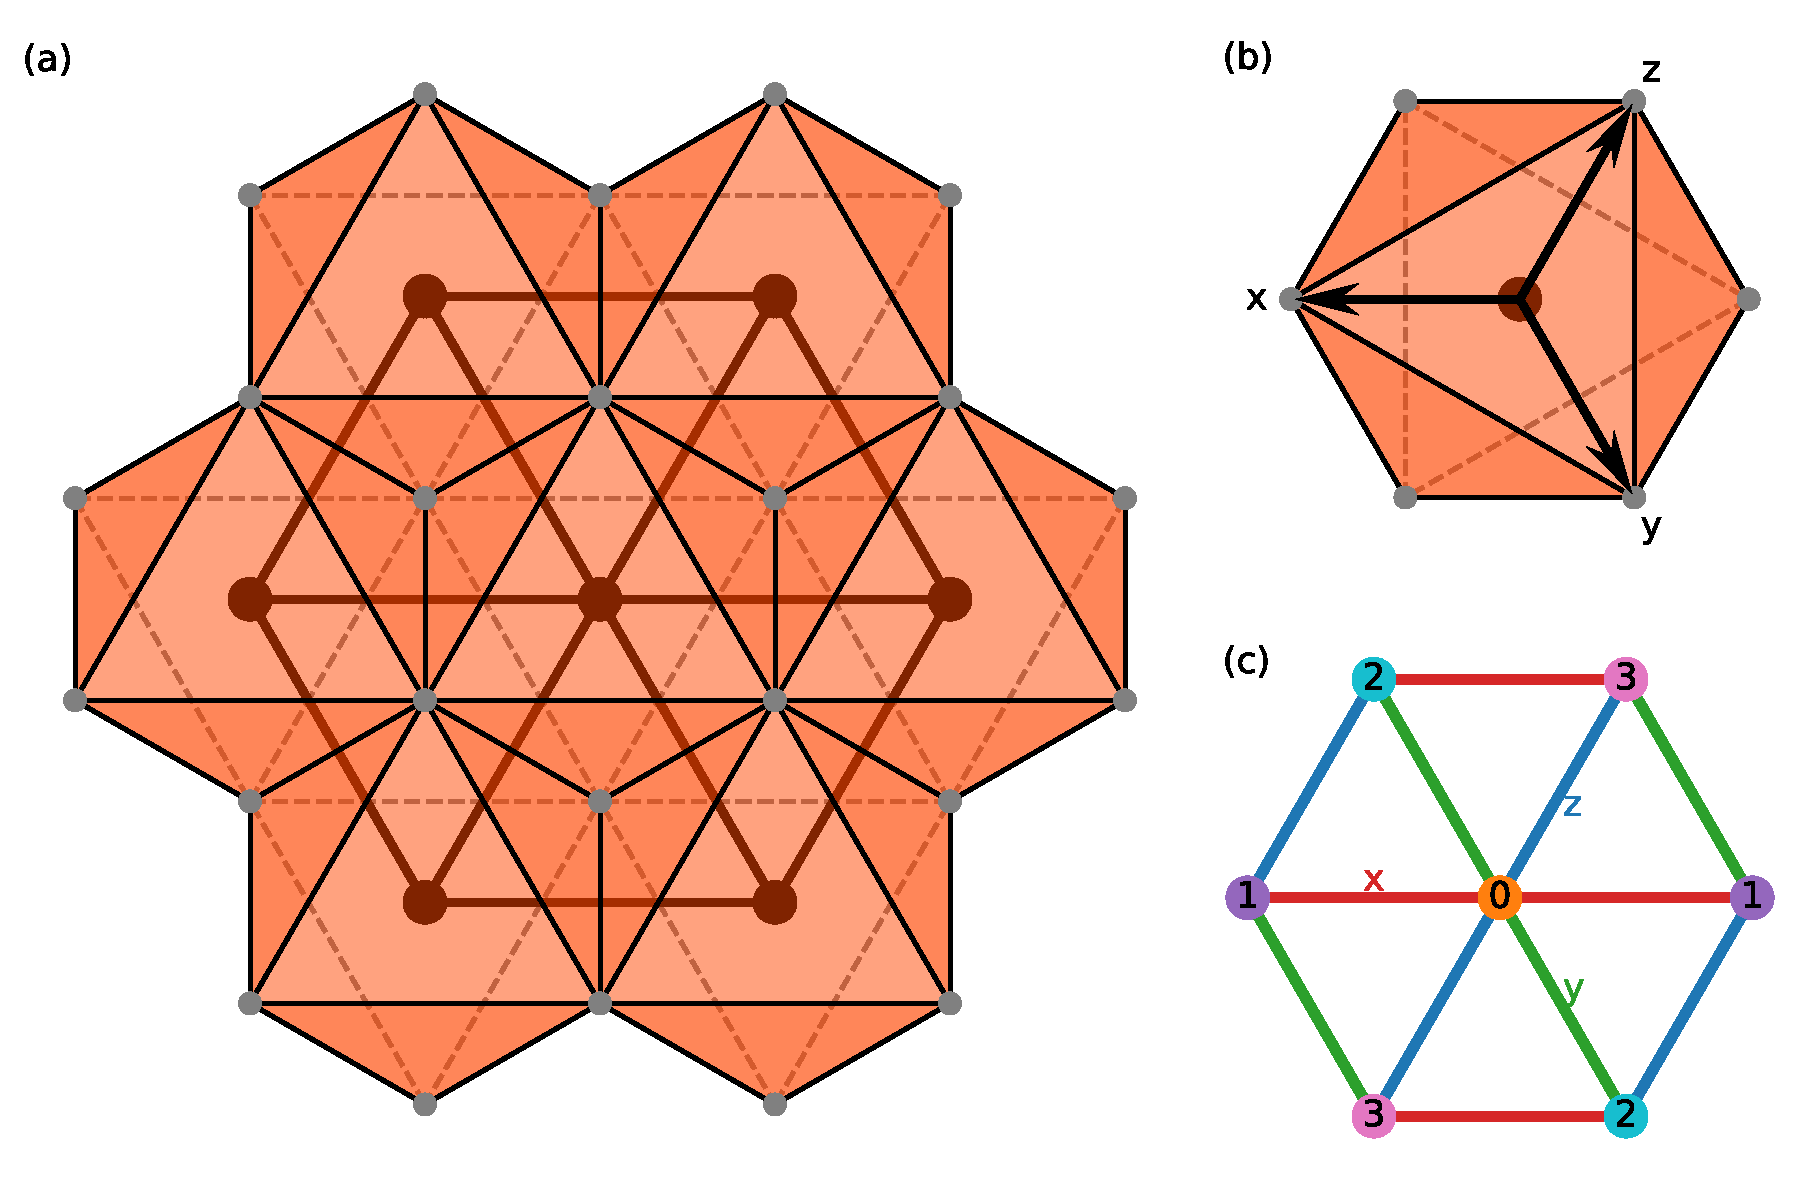
\includegraphics[width=\columnwidth]{Fig1.pdf}
    \caption{\label{fig:ModelDefinition}(Color online) (a) Top view of the triangular lattice of the edge-sharing octahedron. (b) The orientation of the cubic $x$, $y$, $z$ axes with respect to the octahedron. The spin operators $S^x$, $S^y$ and $S^z$ are defined with respect to this reference frame. (c) Three types of the NN bonds on the triangular lattice, namely $\gamma=x, y, z$ colored red, green and blue, respectively. The different colors of the lattice sites label the four sublattices realizing the four-sublattice-transformation, see tha main text for detailed information.}
\end{figure}

The rest of the paper is organized as follows: The classical Monte Carlo and exact diagnoalization (ED) methods are introduced in Sec.~\ref{sec:SectionII}. Section~\ref{sec:SectionIII} discusses the phases of the classical $J-K-\Gamma$ model with the main focus on the direction of the ordered moment of the FM and stripe states. The global phase diagram of the quantum model is presented in Sec.~\ref{sec:SectionIV} along with a discussion of its phases. In Sec.~\ref{sec:SectionV}, we study the moment direction of the quantum FM and stripe states, which provide characteristics to distinguish these phases.

\section{\label{sec:SectionII}Methods}
The full anisotropic Hamiltonian~\eqref{eq:Hamiltonian} is no longer exactly solvable, even for the classical case. One, therefore, either has to rely on approximate analytical method or on numerical techniques. To determine the ground state of the Hamiltonian~\eqref{eq:Hamiltonian}, we employ a combination of classical Monte Cralo simulation and ED calculation. Here, we briefly describe the methods we used. For convenience, we fix the energy scale with $\sqrt{J^2 + K^2 + \Gamma^2}=1$ and parametrize the exchanges using spherical angles $\alpha$ and $\beta$
\begin{equation}
    J = \sin\alpha \sin\beta, \quad
    K = \sin\alpha \cos\beta, \quad
    \Gamma = \cos\alpha \label{eq:Parameters}
\end{equation}
where $\alpha \in [0, \pi]$ and $\beta \in [0, 2\pi]$ to cover the global phase diagram.

\subsection{\label{sec:SectionIIA}Classical Monte Carlo}
\textcolor{red}{A introduction to classical Monte Carlo. To be accomplished $\cdots \cdots$}

\subsection{\label{sec:SectionIIB}Exact Diagonalization}
We perform Lanczos ED calculations of the GS of the Hamiltonian~\eqref{eq:Hamiltonian} on several $4 \times 6$ clusters with periodic boundary conditions (PBC). To detect quantum phase transitions, the second derivatives of the ground state energy, $-\partial^2E_0/\partial\alpha^2$ and $-\partial^2E_0/\partial\beta^2$ were computed and looked for singular features that indicate changes in the ground state characteristics. Phases containing exactly solvable or well-understood points, such as the FM, 120$^\circ$ N\'{e}el, stripe and Dual N\'{e}el can be readily identified. To have a better understanding of the characteristics of the remaining phases, we examine the static magnetic structure factor (SMSF) $S(\bm{Q})$ and dynamic spin excitation spectrum $A(\bm{k}, \omega)$ of these phases. $S(\bm{Q})$ and $A(\bm{k}, \omega)$ are defined as follow:
\begin{subequations}
    \begin{align}
        & S(\bm{Q}) = \frac{1}{N} \sum_{ij} \langle \Omega | \bm{S}_i \bm{\cdot} \bm{S}_j | \Omega \rangle e^{i \bm{Q} \bm{\cdot} (\bm{R}_i - \bm{R}_j)} \label{eq:SMSF} \\
        & A(\bm{k}, \omega) = -\frac{1}{\pi} \text{Im} G(\bm{k}, \omega) \label{eq:Akomega} \\
        & G(\bm{k}, \omega) = \frac{1}{N} \sum_{ij} G_{ij}(\omega) e^{i \bm{k} \cdot (\bm{R}_i - \bm{R}_j)} \\
        & G_{ij}(\omega) = \langle \Omega | S_i^{+} \frac{1}{\omega + i\eta - H + E_0} S_j^{-} | \Omega \rangle \label{eq:GreenFunction}
    \end{align}
\end{subequations}
where $| \Omega \rangle$ and $E_0$ are the GS and ground state energy respectively, N is the total number of spins, $\bm{R}_i$ the position of site $i$, and $\eta = 0^+$.

To extract the moment direction of a magnetic ordered phase from a cluster GS, we employ the method developed by Ji\v{r}\'{i} Chaloupka \emph{et  al} \cite{PhysRevB.94.064435}. The basic idea of this method is to measure the probabilities of the exact cluster GS on cluster spin-coherent states with varying moment directions. The cluster spin-coherent state is a direct product of spin-1/2 coherent states on each site $i$
\begin{equation}
    | \Psi \rangle = \bigotimes_{i=1}^N | \theta_i, \phi_i \rangle \label{eq:ClusterCoherentState}
\end{equation}
where the spin-1/2 coherent state
\begin{equation}
    | \theta, \phi \rangle = \mathcal{R}_z(\phi) \mathcal{R}_y(\theta) | \uparrow \rangle = e^{-i \phi S^z} e^{-i \theta S^y} | \uparrow \rangle \label{eq:Spin-1/2CoherentState}
\end{equation}
is fully polaried along the $(\theta, \phi)$ direction. Here the cubic axes are used (see Fig.~\ref{fig:ModelDefinition}(b)), $\theta$ and $\phi$ are the conventional spherical angles, and $S^z | \uparrow \rangle = \frac{1}{2} | \uparrow \rangle$. By calculating the overlap between the exact cluster GS and cluster spin-conherent states, and maximizing the probability $P = | \langle \Psi | GS \rangle|^2$ with respect to $\theta$s and $\phi$s, we can then identify the classical pattern that best fits the exact GS.

\section{\label{sec:SectionIII}Classical Analysis}
To understand the effects of inculding the off-diagonal $\Gamma$ term, we first study the classical $J-K-\Gamma$ model where the spin operators are viewed as unit-vectors in three dimension. On our proceeding, we note that the global phase diagram has been obtained previously by using a combination of Luttinger-Tsiza (LT) and classical Monte Carlo simulations \cite{PhysRevB.92.165108}. Six different magnetic orderings: ferromagnet (FM), stripe, 120$^\circ$ N\'{e}el order, nematic, $\mathbb{Z}_2$ and dual-$\mathbb{Z}_2$ vortex crystal phases were found, see Fig.~2 in Ref~\onlinecite{PhysRevB.92.165108}. Our classical Monte Carlo study give qualitatively the same phase diagram.

\subsection{\label{sec:SectionIIIA}Moment direction of the classcial FM order}
For the classical FM order, all spins are aligned in parallel and the energy of the $J-K-\Gamma$ model per lattice site is given by
\begin{equation}
    E_{FM}^{c} = (3J + K) + 2 \Gamma (v^x v^y + v^y v^z + v^z v^x) \label{eq:EcFM}
\end{equation}
where $v^x$, $v^y$, $v^z$ are the corresponding components of the classical moment vector. On this level, the moment direction of the classical FM state is determined solely by $\Gamma$ and the problem becomes finding the global minimum and maximum of the multi-variable function $f(v^x, v^y, v^z) = v^x v^y + v^y v^z + v^z v^x$ with the constraint $|\bm{v}| = 1$. $f(v^x, v^y, v^z)$ takes maximum value $f_{max}=1$ at $v^x=v^y=v^z=\pm 1/\sqrt{3}$ and minimum value $f_{min}=-0.5$ when the conditions $v^x + v^y + v^z = 0$ and $|\bm{v}| = 1$ are fulfilled. The condition $v^x + v^y + v^z = 0$ specifies a plane that passes the coordinate origin and is perpendicular to the $[111]$ direction. Considering the reference frame shown in Fig.~\ref{fig:ModelDefinition}(b) this is actually the plane of the triangular lattice. That is to say, for $\Gamma > 0$ the ordered moment of the classcial FM state prefers to lie in the lattice plane and when $\Gamma$ is negative, the ordered moment would perpendicular to the lattice plane.

Our classical Monte Carlo simulation found FM ordered state with the right moment direction for majority of the area marked as FM phase (see Fig.~2 in Ref~\onlinecite{PhysRevB.92.165108}) except for the pure $\Gamma$ term. For pure positive $\Gamma$ interaction, apart from the FM order lie in the lattice plane, we also found disordered states which have the same energy as the FM state but no states with lower energy were found. When $\Gamma=-1$, in addition to the FM order perpendicular to the lattice plane, other long-range ordered states which are energetically degenerate with the FM state appear (see Appendix~\ref{apx:AppendixA} for details). Based on these observation, it is reasonable to say that the GS of the classical $\Gamma$ model is highly degenerate though the degeneracy may be lifted by introducing other interactions. For example, a ferromagnetic ($J<0$) Heisenberg interaction would break the degeneracy and select the FM ordered state as the GS. On the other hand, when positive Heisenberg interaction is included, which introduces further frustation to the system, the FM order is unlikely to be the GS. In fact, the classical GS were found to be disordered for $0 < J \ll \Gamma$ and stripe ordered for $0 < J \ll -\Gamma$. As for the disordered phase, when quantum flucations are involved, a quantum spin liquid state may emerge.

\subsection{\label{sec:SectionIIIB}Moment direction of the classcial stripe order}
In the case of stripe order, there are three degenerate spin configurations as illustrated in Fig.~\ref{fig:PhaseDiagram}(b)-(d). For the spin configuration shown in Fig.~\ref{fig:PhaseDiagram}(b), the energy of the model Hamiltonian~\eqref{eq:Hamiltonian} per lattice site is
\begin{eqnarray}
    E_{StripeX}^{c} & = & -(J + K) + 2 K v^x v^x \nonumber \\
        & & +\: 2 \Gamma (v^y v^z - v^z v^x - v^x v^y) \label{eq:EcStripeX}
\end{eqnarray}
and the energy for spin configuration in Fig.~\ref{fig:PhaseDiagram}(c) and \ref{fig:PhaseDiagram}(d) can be obtained by a cyclic permutation $x \rightarrow y \rightarrow z \rightarrow x$. The ordered moment direction of the classical stripe order is determined by the anisotropy parameters $K$ and $\Gamma$. In general ($K,\Gamma \neq 0$), $E_{StripeX}^{c}$ has six extreme points where the first derivatives with respect to $v_x$, $v_y$ and $v_z$ equal zero. Here we give three of them explicitly and the other three are opposite to the given ones
\begin{subequations}
    \label{eq:whole}
    \begin{eqnarray}
        & \bm{v}_0:& \quad v_{0}^{y}=-v_{0}^{z} = 1/\sqrt{2}, \quad v_{0}^{x} = 0 \label{eq:v0} \\
        & \bm{v}_1:& \quad v_{1}^{y}=v_{1}^{z} = f_{1}(K, \Gamma), \quad v_{1}^{x} = g_{1}(K, \Gamma) v_{1}^{y} \label{eq:v1} \\
        & \bm{v}_2:& \quad v_{2}^{y}=v_{2}^{z} = f_{2}(K, \Gamma), \quad v_{2}^{x} = g_{2}(K, \Gamma) v_{2}^{y} \label{eq:v2}
    \end{eqnarray}
\end{subequations}
see Appendix~\ref{apx:AppendixB} for their explicit expressions.

For $\Gamma=0, K>0$, it can be clearly seen from Eq.~\eqref{eq:EcStripeX} that $E_{StripeX}^{c}$ takes minimum value at $v^x = 0$ which means that the stripe order shown in Fig.~\ref{fig:PhaseDiagram}(b) prefers to lie in the $yz$ plane. An infinitesimal positive $\Gamma$ would fix the ordered moment to the $\bm{v}_0$ direction whereas negative $\Gamma$ drives it to the $\bm{v}_1$ direction. When $\Gamma=0, K<0$, the ordered moment would along the $x$-axis to have lowest energy, both positive and negative $\Gamma$ make it deviate from the $x$-axis and point to the $\bm{v}_1$ direction. All these stripe orders with the specific moment direction were found in the corresponding parameter space by our Monte Carlo simulation. However, in the HK limit ($\Gamma=0$), apart from the stripe orders lie in the axis plane, nematic orders which have the same energy were also found in the range $0 \leq |J| \ll K$ (see Appendix~\ref{apx:AppendixA} for details). The GS of the classical HK model near the antiferromagetic Kitaev point ($K=1$) is high degenerate and both positive and negative $\Gamma$ interactions select specific stripe ordered state as the GS.

\section{\label{sec:SectionIV}Global Phase Diagram}
\begin{figure*}
    \centering
    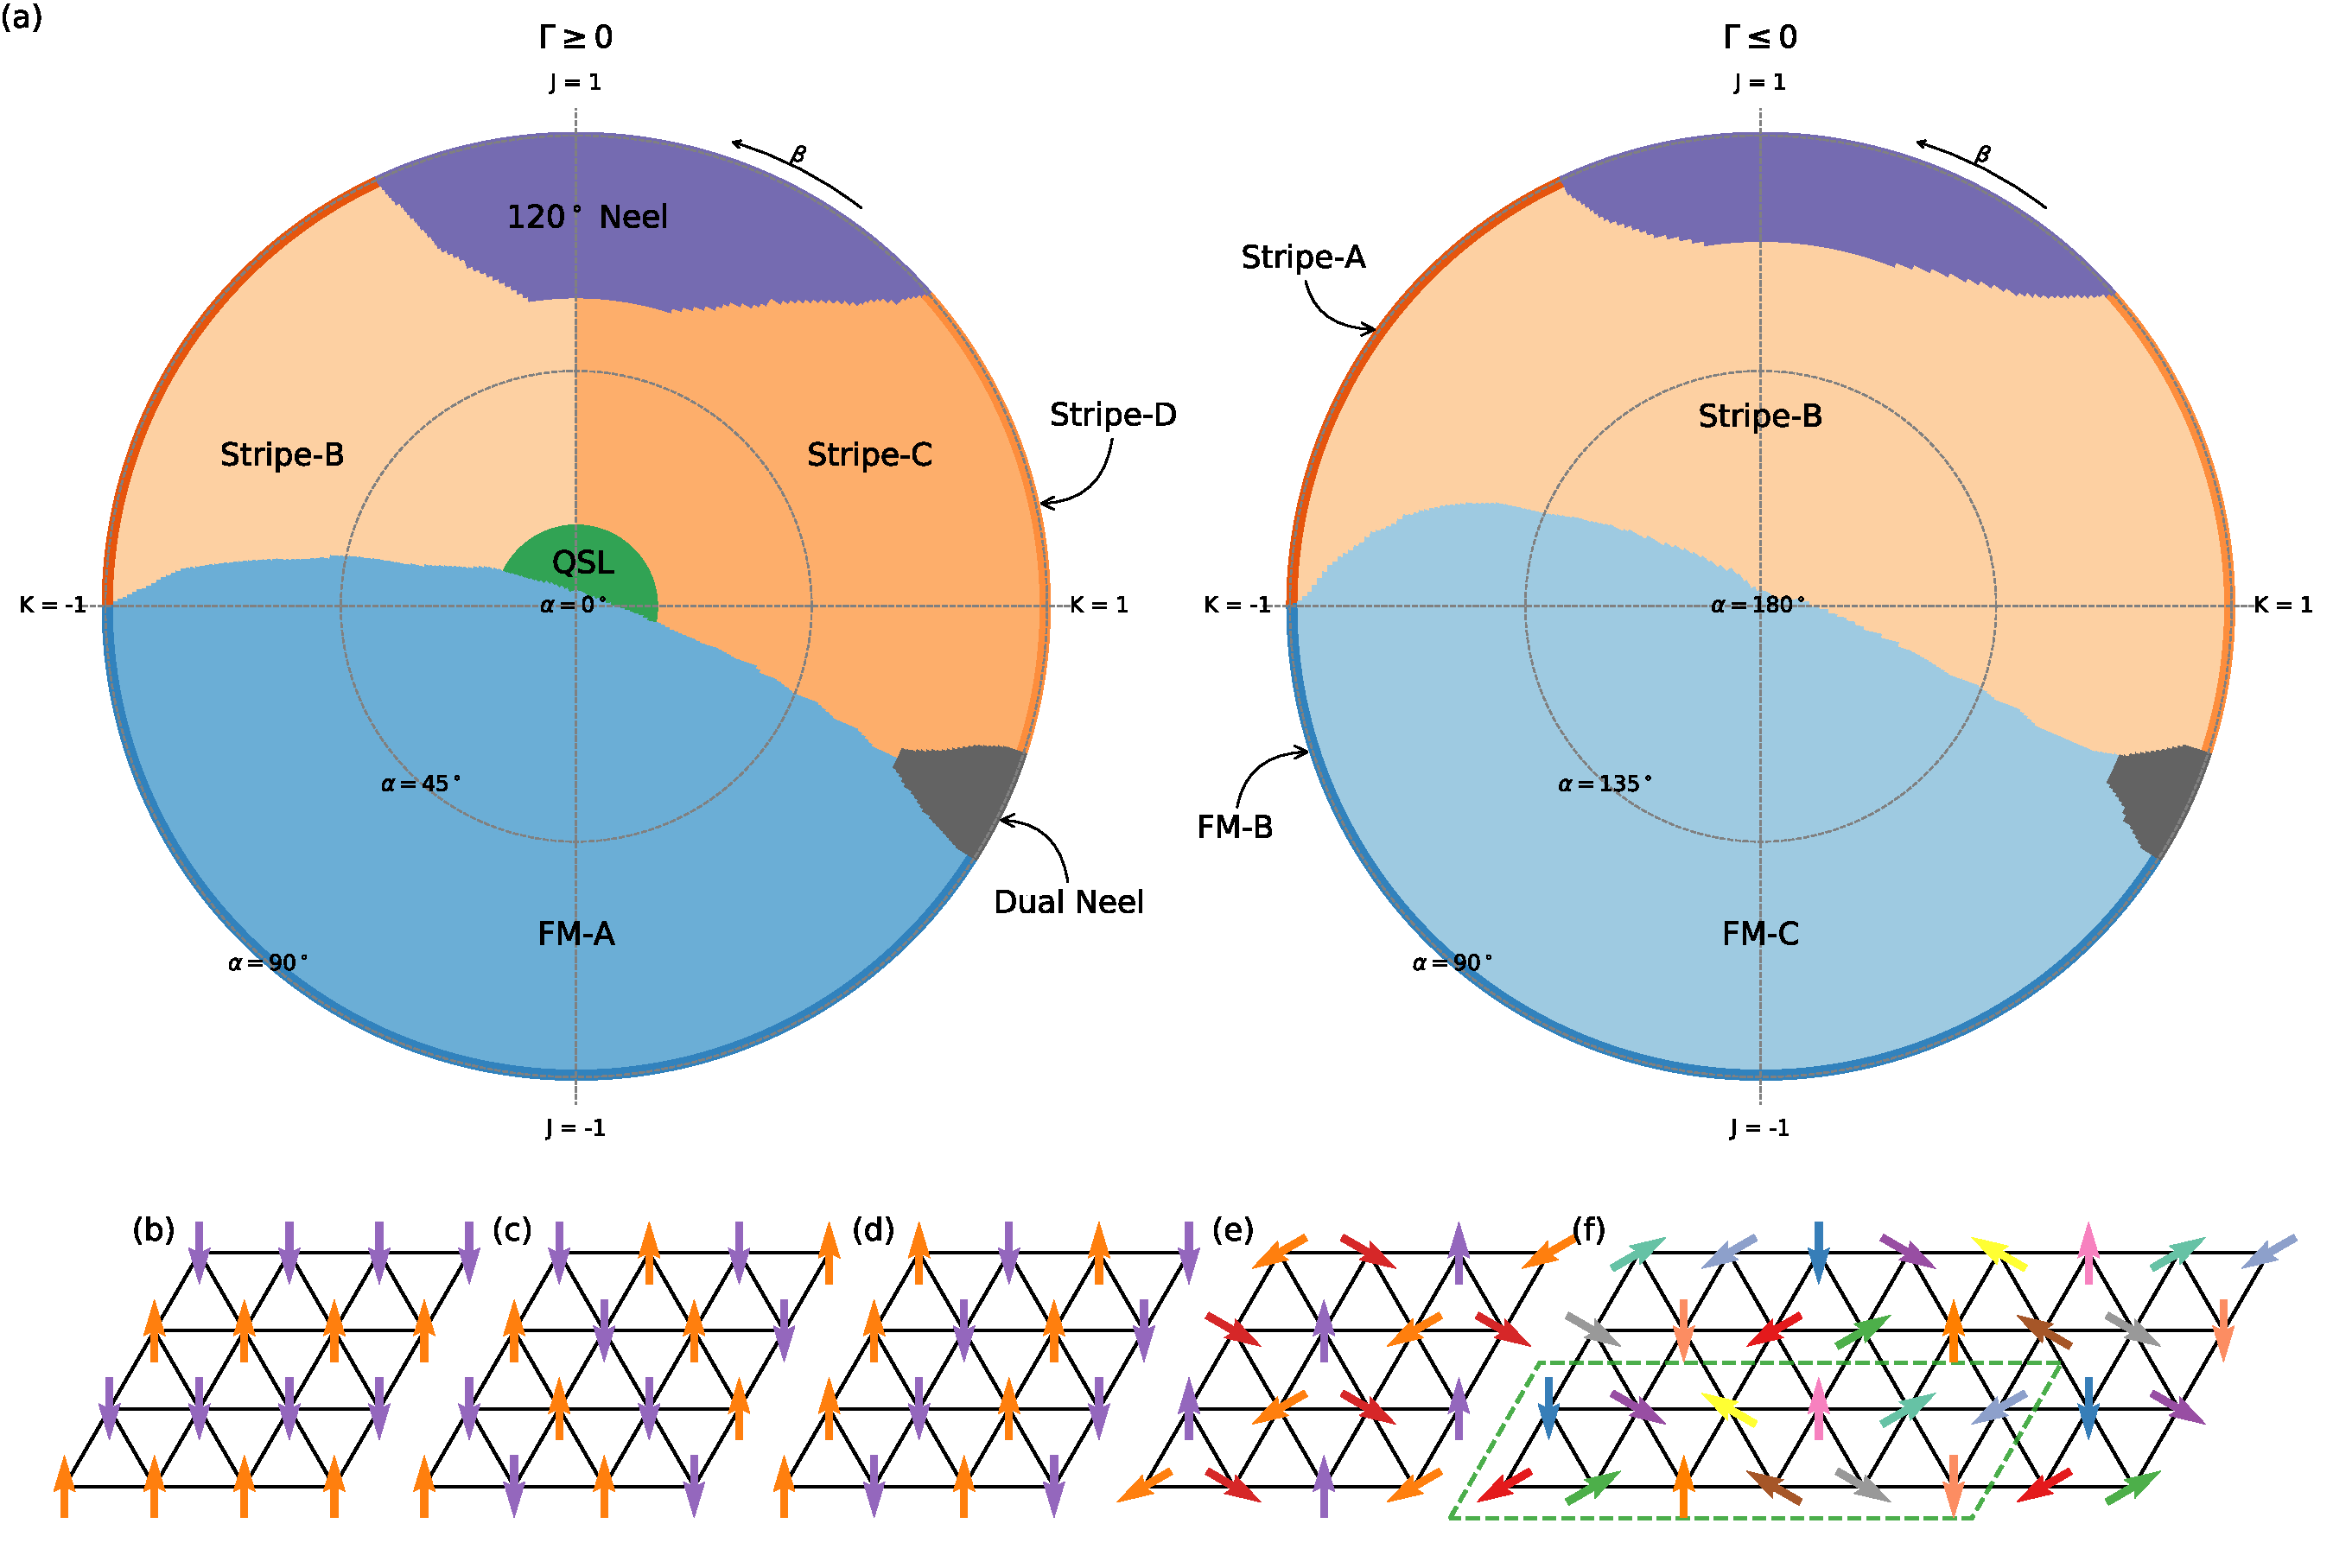
\includegraphics[width=0.96\textwidth]{Fig2.pdf}
    \caption{\label{fig:PhaseDiagram}(Color online) (a) Global phase diagram of the triangular lattice $J-K-\Gamma$ model. The angle $\alpha$ and $\beta$ denote the radial and azimuthal angles, respectively. There are in total ten phases including three different FM phases denoted as FM-A, FM-B and FM-C, four different stripe phases designated as Stripe-A, Stripe-B, Stripe-C and Stripe-D, 120$^\circ$ N\'{e}el, Dual N\'{e}el and a possible quantum spin liquid phase. The three FM phases different from each other in the direction of the ordered moment, and also the four stripe phases are distinguished by their moment directions, see main text for details. (b)-(d) Illustation of the three degenerate spin configurations for all stripe orders. (e) Illustration of the 120$^\circ$ N\'{e}el order. All spins are coplanar and the angles between nearest-neighbor spins are 120$^\circ$. (f) Illustration of the Dual N\'{e}el order. The magnetic unit cell include 12 lattice sites as marked by the green dashed parallelogram.}
\end{figure*}

In this section, we turn to study the quantum phases in the $J-K-\Gamma$ model Hamiltonian. We consider a $4 \times 6$ cluster with PBC that has been used previously to study the KH model on triangular lattice \cite{KaiLi2015}. The resulting phase diagrams for $\Gamma \geq 0$ and $\Gamma \leq 0$ are presented in Fig.~\ref{fig:PhaseDiagram}(a). The phase boundaries are obtained from the location of singular features in $-\partial^2E_0/\partial\alpha^2$ and $-\partial^2E_0/\partial\beta^2$. The quantum phase diagram is closely resemble to the classical result in Ref~\onlinecite{PhysRevB.92.165108} except for the small green area near $\Gamma=1$ which does not appear in the classical phase diagram.

\subsection{\label{subsec:HKLimit}Phases in the HK limit ($\Gamma=0$)}
For pure Heisenberg model ($K=\Gamma=0$), the GS is ferromagnet for $J<0$ and 120$^\circ$ N\'{e}el state for $J>0$. As for the HK ($\Gamma=0$) model, by virtue of the existence of the so-called four-sublattice-transformation (FST) \cite{PhysRevB.89.014414}, two more magnetic ordered phases can be identified. Specifically, FST is a spin rotation transformation which divide the triangluar lattice into four sublattices (see Fig.~\ref{fig:ModelDefinition}(c)) and introduce the rotated spin operators $\bm{S}^{'}$
\begin{align*}
    & \bm{S}_{0}^{'} = \bm{S}_{0}& \quad \text{for sublattice 0} \\
    & \bm{S}_{1}^{'} = (S_1^x, -S_1^y, -S_1^z)& \quad \text{for sublattice 1} \\
    & \bm{S}_{2}^{'} = (-S_2^x, S_2^y, -S_2^z)& \quad \text{for sublattice 2} \\
    & \bm{S}_{3}^{'} = (-S_3^x, -S_3^y, S_3^z)& \quad \text{for sublattice 3}
\end{align*}
The resulting Hamiltonian $H^{'}(\bm{S}^{'})$ has the same form as the original Hamiltonian albeit with different model parameters $J^{'} = -J$ and $K^{'} = 2J + K$. For the spherical angles defined in Eq~\eqref{eq:Parameters}, the mapping takes the form $tan\beta^{'}=-sin\beta/(2sin\beta + cos\beta)$. When $\beta=\pi - arctan\frac{1}{2}$, the FST maps the Hamiltonian~\eqref{eq:Hamiltonian} to FM Heisenberg model of the rotated spin operators $\bm{S}^{'}$. Thus, transformating back to the original spin basis, a collinear stripe order can be obtained. Similarly, a noncollinear spiral order (dual N\'{e}el) at $\beta=-arctan\frac{1}{2}$ can be obtained from the 120$^\circ$ N\'{e}el order (see Fig.~\ref{fig:PhaseDiagram}(e) and (f)).

Apart from these well-established phases, the phase near the AF Kitaev point (i.e., $K=1$) has been proposed to be a chiral SL at the mean field level \cite{KaiLi2015} or a nematic phase in the quantum limit from DMRG calculation \cite{PhysRevB.91.155135}, however, a more recent study suggests that a stripe state is more likely to be the GS \cite{PhysRevX.9.021017}. To determine the GS of HK model in this area, we calculate the SMSF at $K=1$ and the resulting profile is shown in Fig.~\ref{fig:StructureFactors}(c). It is clear from Fig.~\ref{fig:StructureFactors}(c) that the SMSF peaked at the midpoints of the first BZ boundary (i.e., M-points) which is a typical characteristic of stripe ordered states.

To have further insight into these phases, we adopt the method introduced in Ref~\onlinecite{PhysRevB.94.064435} to extract the moment directions for some of these phases. For pure Heisenberg model, the FM state is spin rotational invariant and the ordered moment can point any direction. The easy axis Kitaev interaction breaks the accidental spin rotational symmetry, pinning the orderings to the axis direction (i.e., $x$, $y$, $z$ direction). In other words, the ordered moment of the FM-B phase is in the direction of the $x,y,z$-axis. As for stripe ordered states, there are three degenerate patterns in real space as shown in Fig.~\ref{fig:PhaseDiagram}(b)-(d) and the ordered moment is locked to the orientation of the stripe pattern. Since the cluster spin-coherent state is captured only by a single pair of $(\theta, \phi)$ for collinear states (in our case, these are FM and stripe), it is easy to determine the direction of the ordered moment by inspecting the probability map $P(\theta, \phi) = | \langle \Psi (\theta, \phi) | GS \rangle |^2$. For brevity, we only construct cluster spin-coherent state based on the stripe pattern shown in Fig.~\ref{fig:PhaseDiagram}(b) and the resulting probability maps for the representative model parameters of the Stripe-A and Stripe-D phase are shown in Fig.~\ref{fig:Proabilities}(c) and Fig.~\ref{fig:Proabilities}(f). The probability map for the Stripe-A phase has high intensity at $(\pi/2, 0)$ and $(\pi/2, \pi)$ which means the ordered moment would along the $x$-axis direction. The Stripe-A phase is connected to the FM-B phase through FST and the spins are supposed to along the $x$-axis for stripe pattern in Fig.~\ref{fig:PhaseDiagram}(b) from classical considerations, our ED results show that this situation also applies at quantum limit. On the other hand, the relative high intensity of $P(\theta, \phi)$ at $(0, 0)$ and $(\pi/2, \pm\pi/2)$ in Fig.~\ref{fig:Proabilities}(f) indicates that the ordered moment pointing to the $y$ and $z$-axis direction. The small $P_{max}$ of about 3\% can be partly attributed to the cluster GS being a superposition of three possible stripe patterns and every pattern has four ordered moment direction (i.e., $\pm y$, $\pm z$ for Fig.~\ref{fig:PhaseDiagram}(b), $\pm x$, $\pm z$ for Fig.~\ref{fig:PhaseDiagram}(c), $\pm x$, $\pm y$ for Fig.~\ref{fig:PhaseDiagram}(d)), more importantly it a signature of large quantum flucations in the ground state. It is worth to note that even the GS of the classical AF Kitaev model was identified to be highly degenerate involving nematic and stripe ordered states, our ED results favor the idea that quantum flucations would select stripe ordered states as GS out of an otherwise infinitely degenerate manifold of classical states. This selection of states among a continuum is the so called "order-from-disorder" mechanism previously emphasized by Villain and Henley in the context of the square lattice XY model \cite{PhysRevLett.62.2056} and by Oguchi \emph{et al.,} in the case of fcc antiferromagnet \cite{JPSJ.54.4494}.

In a word, for the HK model, apart from these well established phases, our ED calculations provide evidence that the GS of the model near the AF Kitaev point is stripe ordered states. However, Stripe-D different from Stripe-A in the direction of the ordered moment direction. To be specific, for a certain spin pattern, the ordered moment would along only one of the $x, y, z$-axis direction in the Stripe-A phase and point to the other two axes directions for the Stripe-D phase.

\begin{figure}
    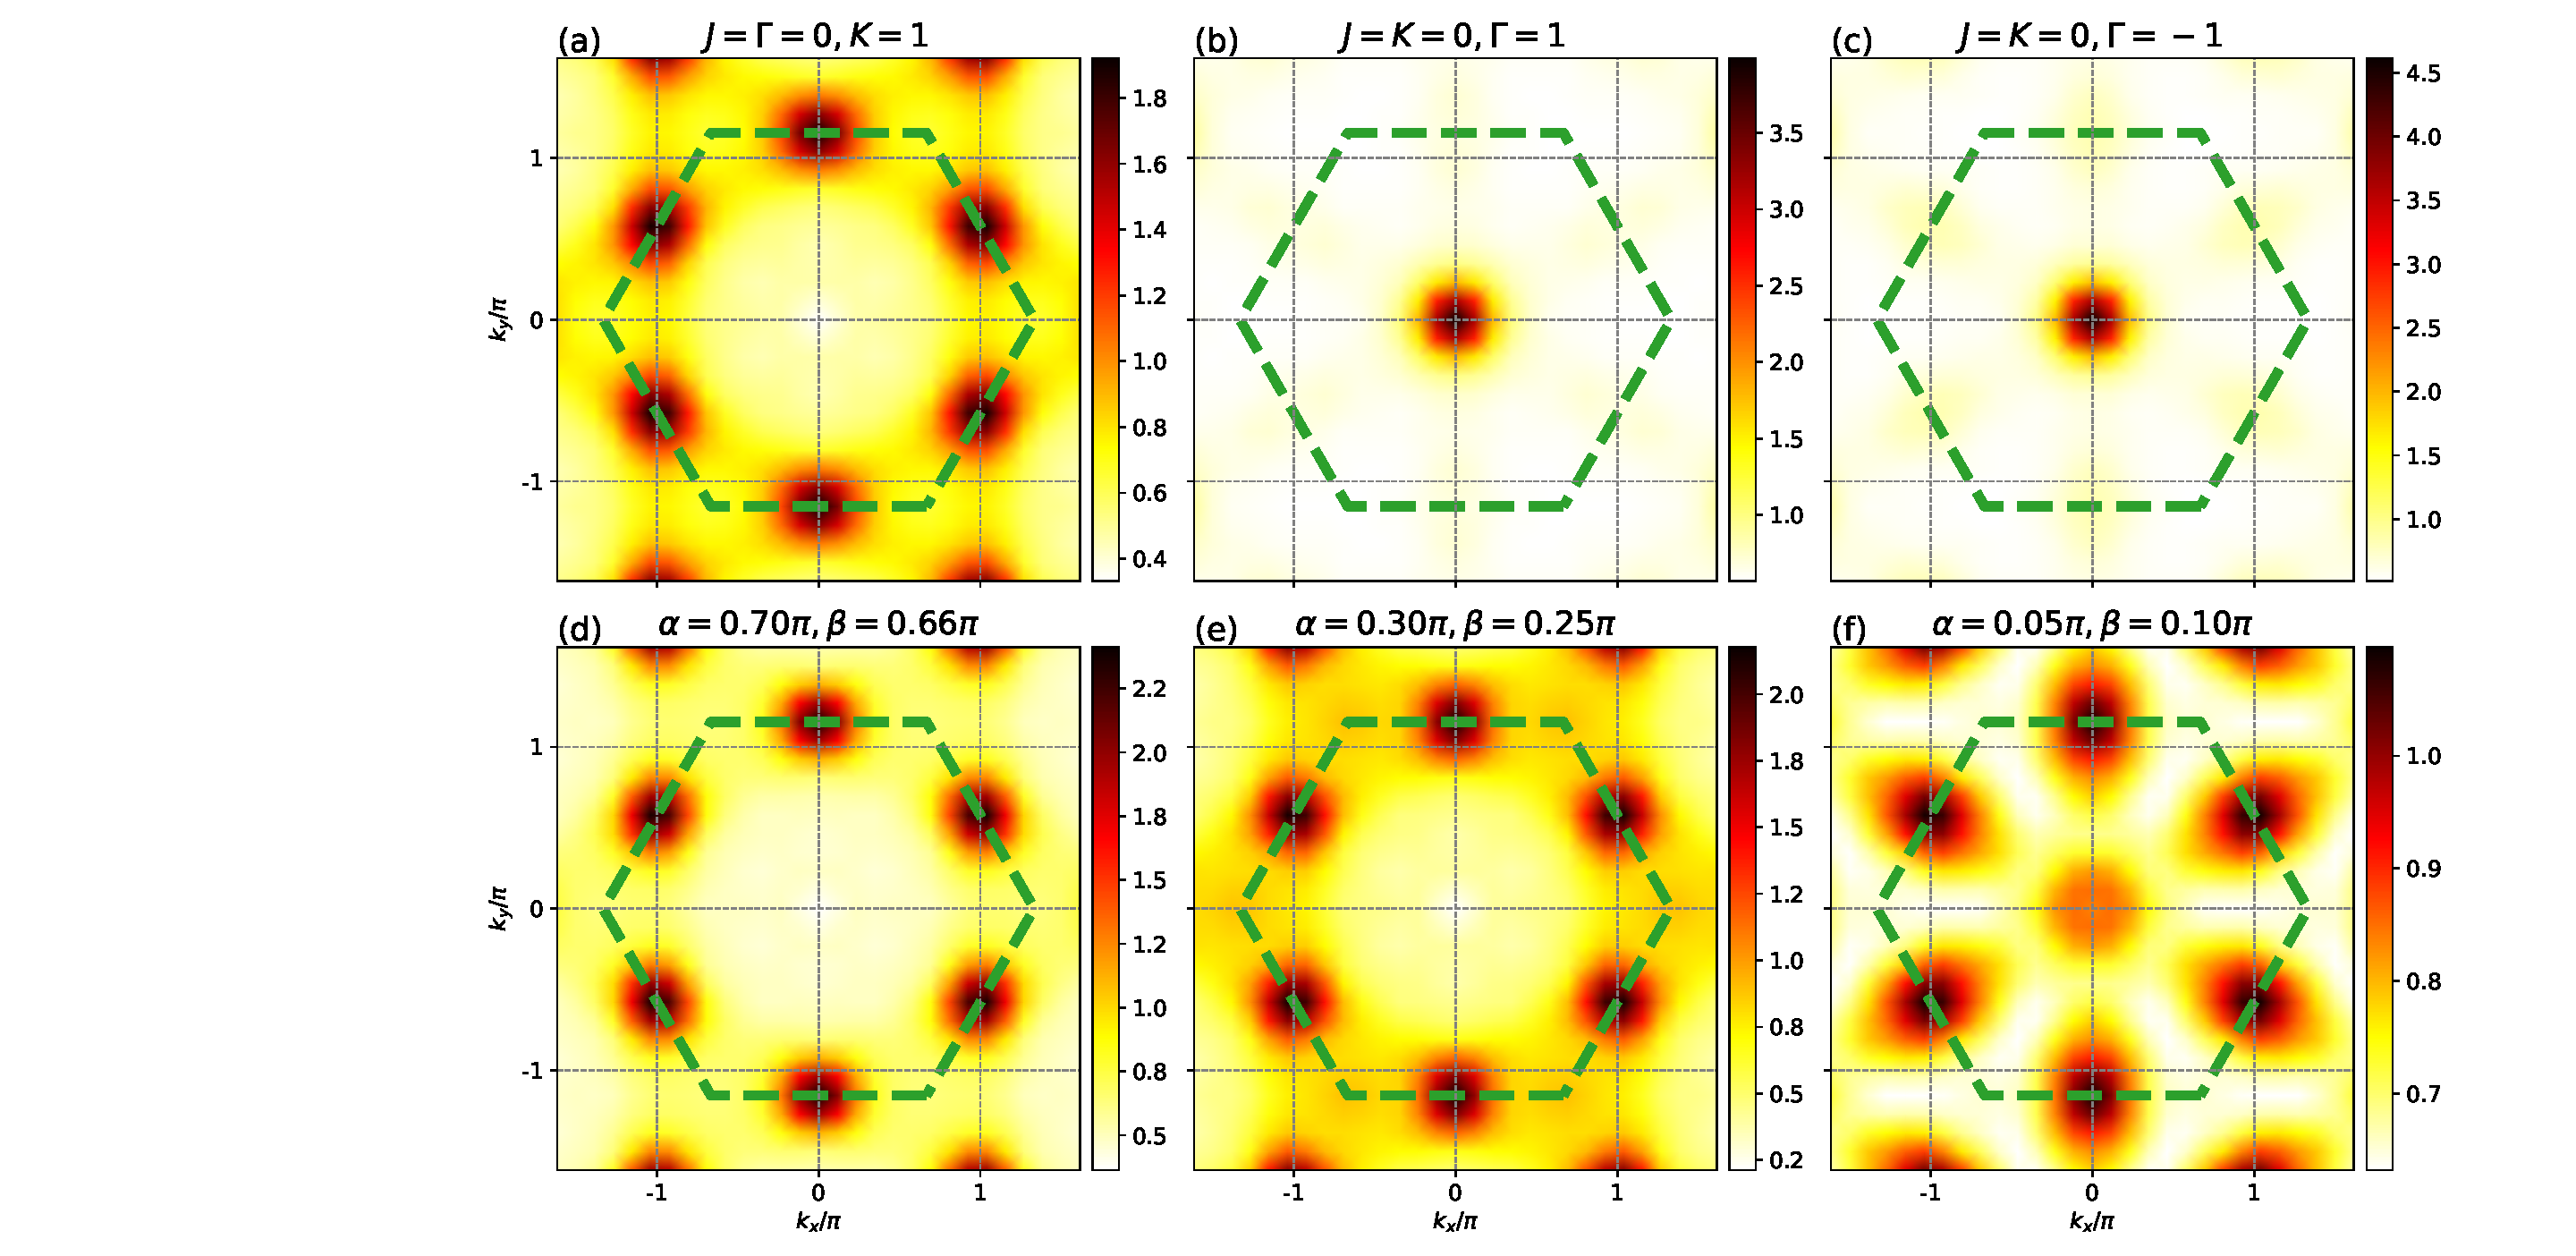
\includegraphics[width=0.45\textwidth]{Fig3.pdf}
    \caption{\label{fig:StructureFactors}(Color online) SMSF for different model paramters. The green dashed lines marks the first BZ corresponding to the triangular lattice.}
\end{figure}
\begin{figure}
    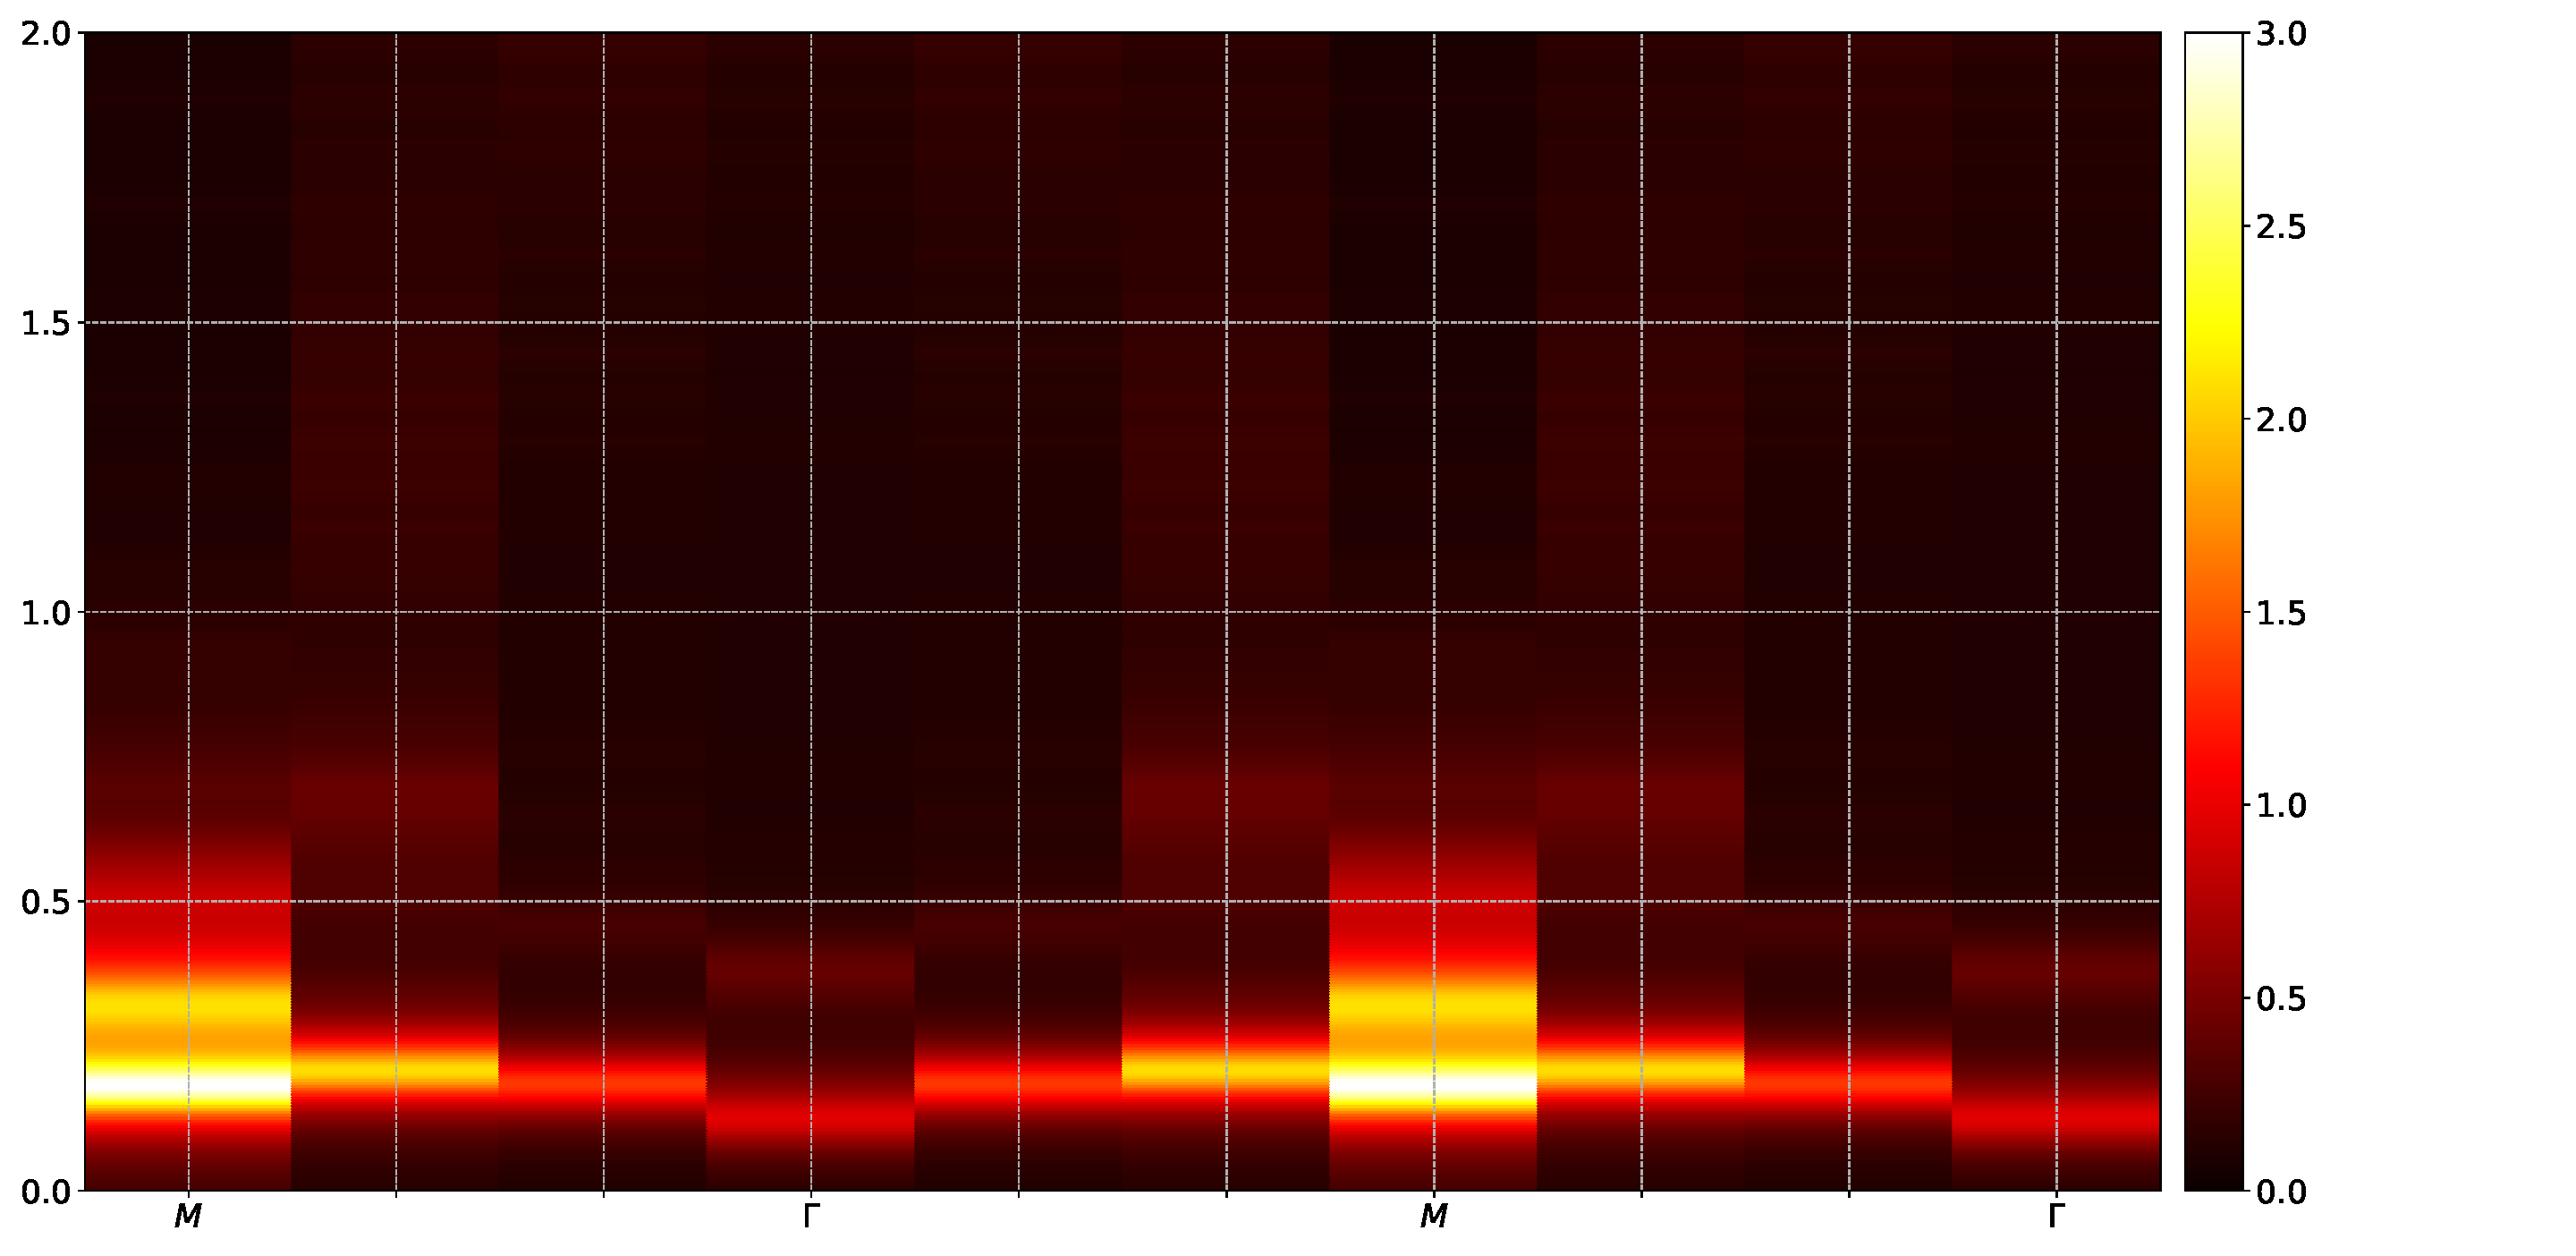
\includegraphics[width=0.45\textwidth]{Fig5.pdf}
    \caption{\label{fig:Proabilities}(Color online) Map of the probabilities of the cluster spin-coherent state given by Eq.~\eqref{eq:ClusterCoherentState} in varies exact cluster GS. The radial and polar coordinate gives the angles $\theta$ and $\phi$, which are spherical angles with respect to the reference frame shown in Fig.~\ref{fig:ModelDefinition}(c). The green dashed lines and solid circles mark the ordered moment direction for the classical states, see main text for details. (a)-(b) Probability maps for the FM states in the FM-A and FM-C phase, respectively. (c)-(f) Proability maps for the stripe states in the Stripe-A, Stripe-B, Stripe-C and Stripe-D phase, respectively.}
\end{figure}

\subsection{\label{subsec:GammaEffects}Effects of the $\Gamma$ term}
When the off-diagonal $\Gamma$ term is included, the FST is no longer valid. To study the nature of these remaining phases, we calculate the SMSF for some representative model paramters, as shown in Fig.~\ref{fig:StructureFactors}. For pure $\Gamma$ model, see Fig.~\ref{fig:StructureFactors}(a) and (b), the peak of the SMSF locates at the center of first Brillouin Zone (BZ) which is a typical characteristic of the FM order. Bases on this observation, we propose the areas containing the $\Gamma=\pm 1$ points in the global phase diagram to be FM ordered phases (i.e., FM-A, FM-C). To further confirm our hypothesis, we construct cluster spin-coherent states with all the spins are polarized along the $(\theta, \phi)$ direction. By inspecting the probability map $P(\theta, \phi)$, we can measure the presence of the cluster spin-coherent states in the exact cluster GS. The resulting probability maps are shown in Fig.~\ref{fig:Proabilities}(a) and \ref{fig:Proabilities}(b). The large overlap between the exact cluster GS and FM ordered cluster spin-coherent state provides solid evidence that the corresponding areas are FM phases. For the FM-A phase, the probability map reveals the moment being constrained to the lattice plane (marked by the green dashed line in Fig.~\ref{fig:Proabilities}(a)) with all directions degenerate. The probability map for the FM-C phase is clearly peaked at the direction perpendicular to the lattice plane (marked by the green solid circle in \ref{fig:Proabilities}(b)). The ground states of the quantum model in these areas are similar to their classical analogue except for the pure $\Gamma$ model. For $\Gamma=1$, the GS of the classical model is highly degenerate including FM ordered states and states with no long range order. However, for the quantum model, quantum flucations select the FM ordered states lie in the lattice plane as GS out of an otherwise infinitely degenerate manifold of classical states. Similarly, the degeneracy for the classical model at $\Gamma=-1$ is lifted by quantum flucations and the FM state perpendicular to the lattice plane is selected as the GS. In the HK limit, the GS of the model near the $J=-1$ point is FM state and the ordered moment is fixed to the $x,y,z$-axis direction by the Kitaev interaction. When an infinitesimal $\Gamma$ interaction is introduced, positive couplings drive the ordered moment to the lattice plane and negative couplings pinning the ordered moment to be perpendicular to the lattice plane.

For these areas marked as Stripe-B and Stripe-C in the global phase diagram, the representative SMSF profiles are shown in Fig.~\ref{fig:StructureFactors}(e) and Fig.~\ref{fig:StructureFactors}(d). For all of these model parameters, the SMSF peaked at the M-points indicating stripe ordered GS in these areas. To test the presence of the classical stripe ordered states, we construct cluster spin-coherent states based on the spin pattern shown in Fig.~\ref{fig:PhaseDiagram}(b) and the resulting probability maps are shown in Fig.~\ref{fig:Proabilities}(d) and Fig.~\ref{fig:Proabilities}(e). When $\alpha=0.7\pi,\beta=0.66\pi$, the probability takes maximum value at the direction determined by Eq.~\eqref{eq:v1}, whereas $P(\theta, \phi)$ is clearly peaked at the direction given by Eq.~\eqref{eq:v0} for $\alpha=0.3\pi, \beta=0.25\pi$. Considering the overall reduction factor of $\frac{1}{6}$ due to the six possible stripe states being superposed in the exact cluster GS, it is reasonable to say that the stripe ordered ground states for the classical $J-K-\Gamma$ model in these areas persist in the quantum limit and the ordered moments of the quantum states coincide with their classical analogue. The reduced probabilities $P_{max} < \frac{1}{6}$ may be attributed to quantum flucations. In the HK limit, there exist a stripe phase (i.e., Stripe-A) when $J>0, K<0$ and the ordered moment along the $x,y,z$-axis direction. When an infinitesimal $\Gamma$ interaction is included, both positive and negative couplings tilting the ordered moment orientation away from the cubic axes directions, yielding the Stripe-B phase. The ordered moment orientation of the Stripe-B phase is given by Eq.~\eqref{eq:v1} and its equivalents (see Appendix~\ref{apx:AppendixB} for details).
%When $\Gamma \rightarrow 0^{+}$ or $\Gamma \rightarrow 0^{-}$, the direction determined by Eq.~\eqref{eq:v1} tend to be the same as the $x$-axis direction which means the phase transition from positive $\Gamma$ to negative $\Gamma$ is continuous.%
As for the Stripe-D phase near the AF Kitaev point, the effect of the $\Gamma$ term is again tilting the ordered moment away from the cubic axes directions though the effects for positive and negative couplings are different. An infinitesimal positive $\Gamma$ interaction changes the ordered moment orientation from the cubic axes directions to the direction specified by Eq.~\eqref{eq:v0} and its equivalents (see Appendix~\ref{apx:AppendixB} for details). On the other hand, when an infinitesimal negative $\Gamma$ interaction is introduced, the ordered moment is rotated to the direction determined by Eq.~\eqref{eq:v1} and its equivalents.

\begin{figure}
    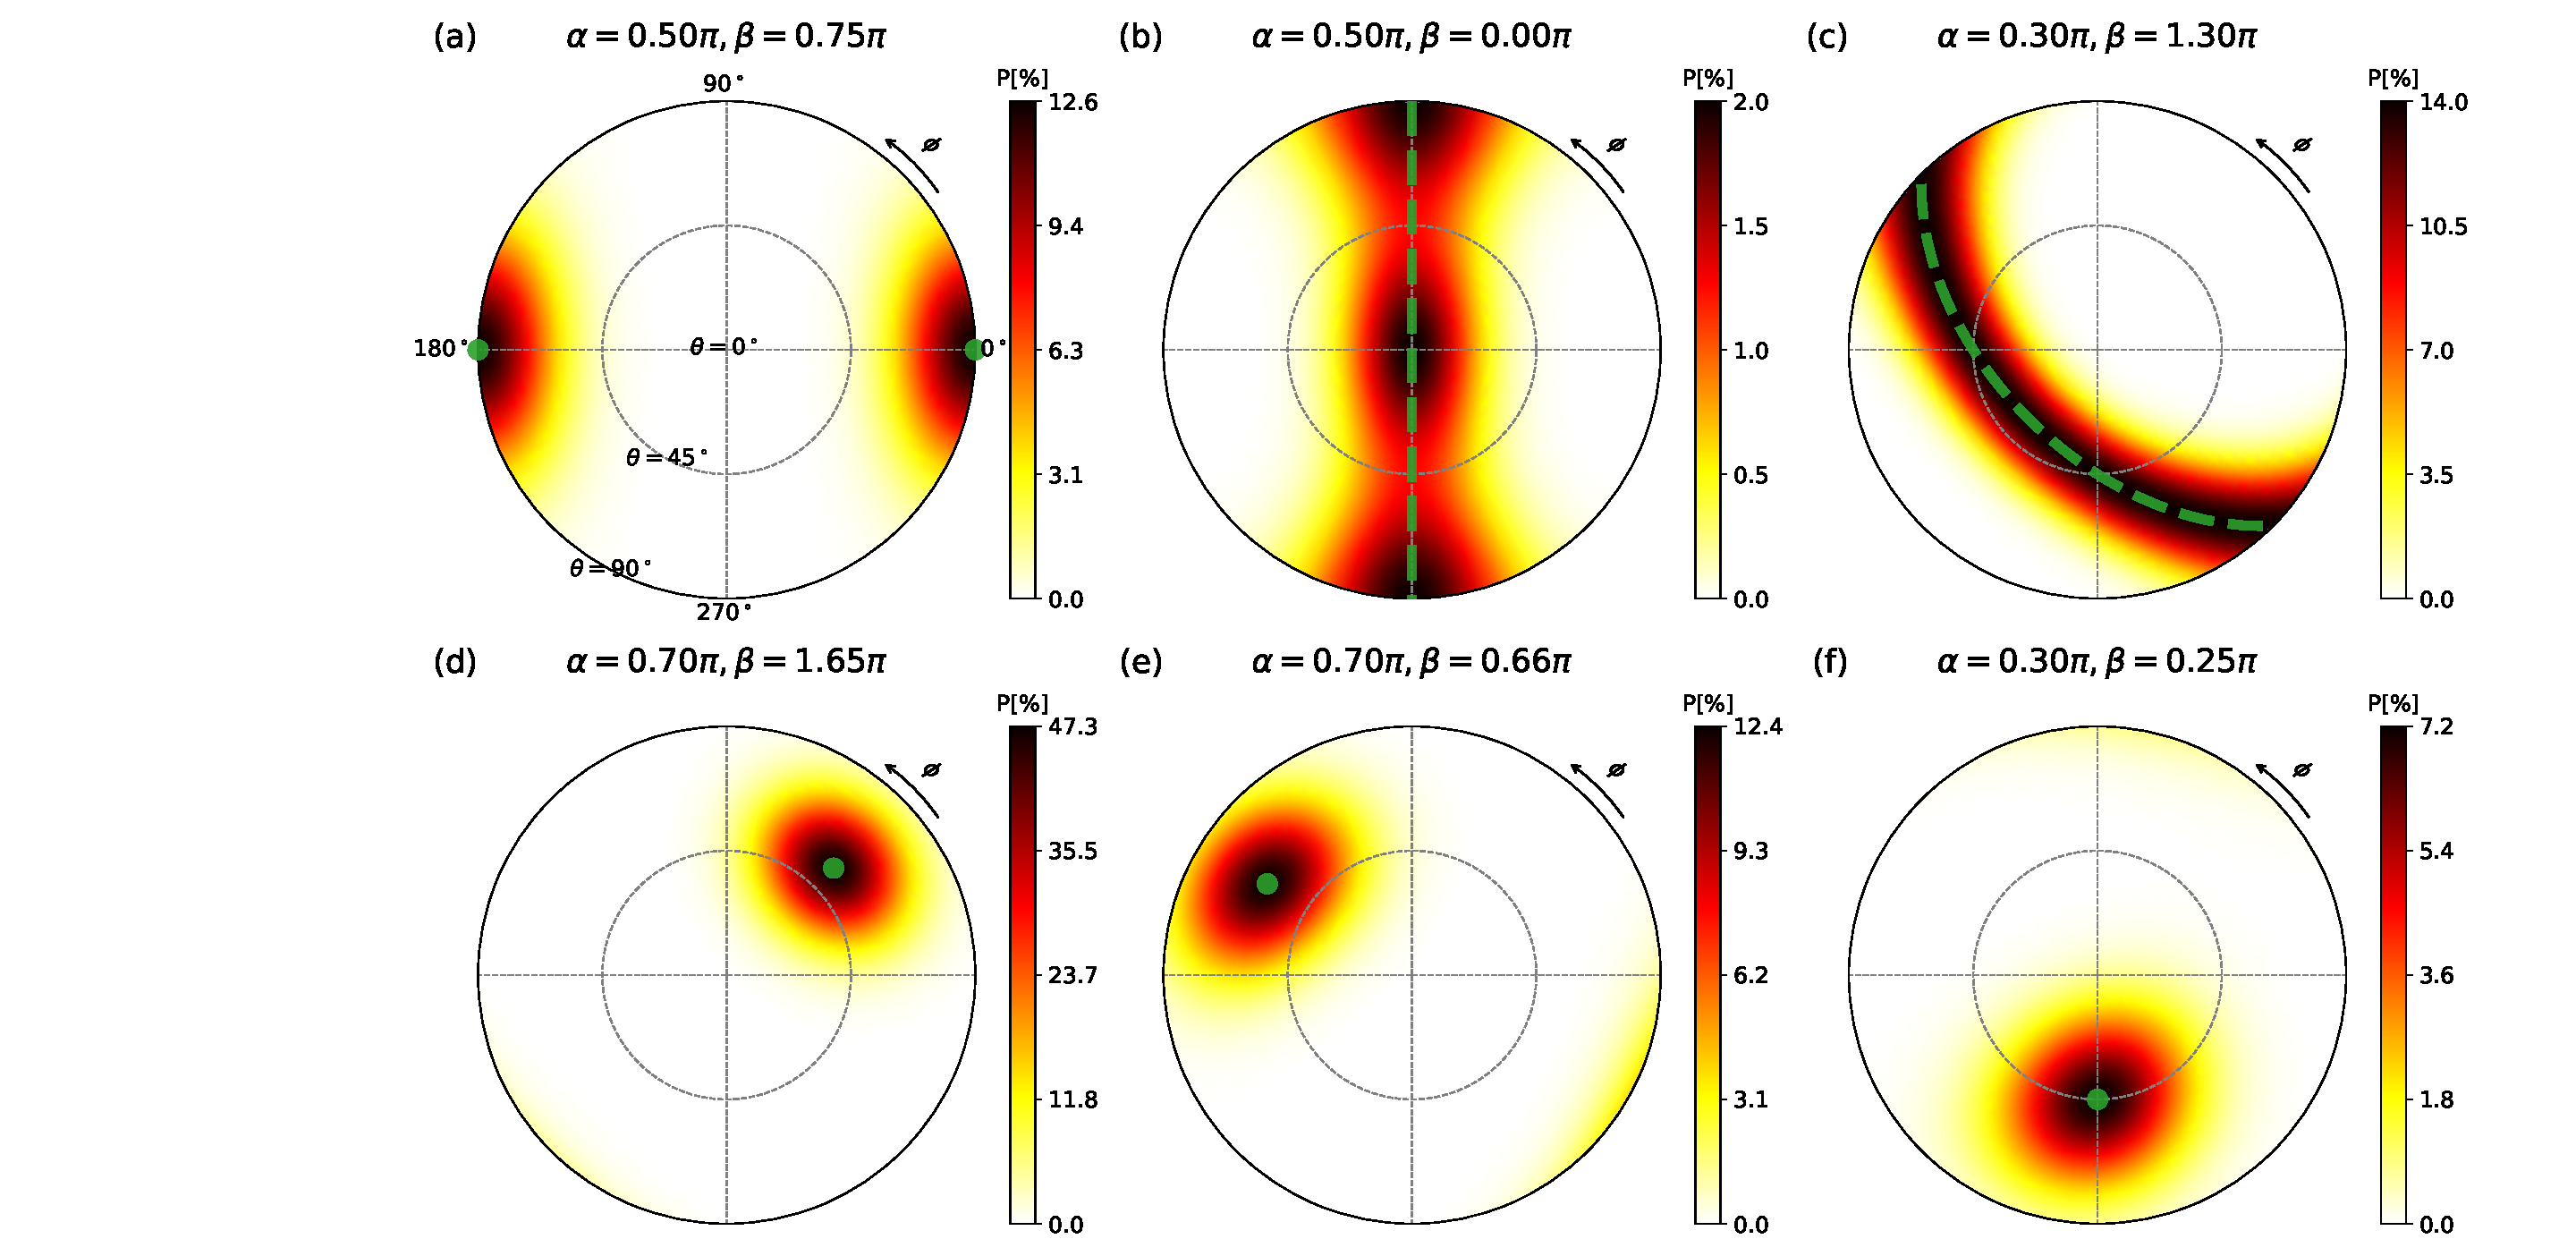
\includegraphics[width=0.45\textwidth]{Fig4.pdf}
    \caption{\label{fig:Spectrum}(Color online) (a) The k-points in the first Brillouin zone corresponding to a 4 $\times$ 6 cluster with 4 lattice sites along the $x$-bond direction and 6 lattice sites along the $y$-bond direction. (b) Spin excitation spectrum for $\alpha=0.05\pi,\beta=0.10\pi$. The $A(\bm{k}, \omega)$ is draw along the path shown in (a).}
\end{figure}

Apart from these single-$\mathbf{Q}$ phases, we also identify a multi-$\mathbf{Q}$ phase, see the green area in Fig.~\ref{fig:PhaseDiagram}(a). For $J$, $K$, $\Gamma$ in this area, the SMSF has high intensities at both the center and M-points of the first BZ. Fig.~\ref{fig:StructureFactors}(f) is a typical SMSF profile of this phase. To have further understanding of the characteristics of this phase, we also calculate the spin excitation spectrum and a typical $A(\mathbf{k}, \omega)$ profile is shown in Fig~\ref{fig:Spectrum}(b). The high intensities at both the center and M-points of the first BZ is consistent with the SMSF data. Moreover, there are continuum spectrum at high energy which is a characteristic of QSL. However, the $A(\mathbf{k}, \omega)$ does not have intensities at $\omega = 0$ which indicates the system described by the corresponding model Hamiltonian is gapped. Combined with all of the above results, we propose the GS of quantum $J-K-\Gamma$ model at the green area is a gapped QSL.

\section{\label{sec:SectionV}Summary}
In summary, by using classical Monte Carlo simulation and exact diagnoalization we map out the global phase diagram of both the classical and quantum $J-K-\Gamma$ model. The global phase diagram of the quantum model is analogus to its classical counterpart except a small area of QSL near the antiferromagetic $\Gamma$ point. We propose the QSL to be gapped based on the spin excitation spectrum. Apart from this QSL phase, we also provide detailed description of the distinctions between those collinear phases. Especially, we propose the GS of the antiferromagetic Kitaev model to be a stripe ordered state and the ordered moment along the $x, y, z$-axis direction.

\begin{acknowledgments}
    \textcolor{red}{Acknowledgements.  To be accomplished $\cdots \cdots$}
\end{acknowledgments}


% The following are the Appendixes of this article
\newpage
\appendix

\section{\label{apx:AppendixA}Classical ground states for some special model parameters}

\subsection{$J=K=0, \Gamma=1$}
For pure antiferromagetic $\Gamma$ model, the classical ground state is highly degenerate including FM state as well as states with no long range order. The ordered moment of the FM state lie in a plane that passes the coordinate origin and is perpendicular to the $[111]$ direction. Fig.~\ref{fig:GSForPositiveGamma} show a typical spin configuration of those disordered states that have the same energy as the FM state.
\begin{figure}
    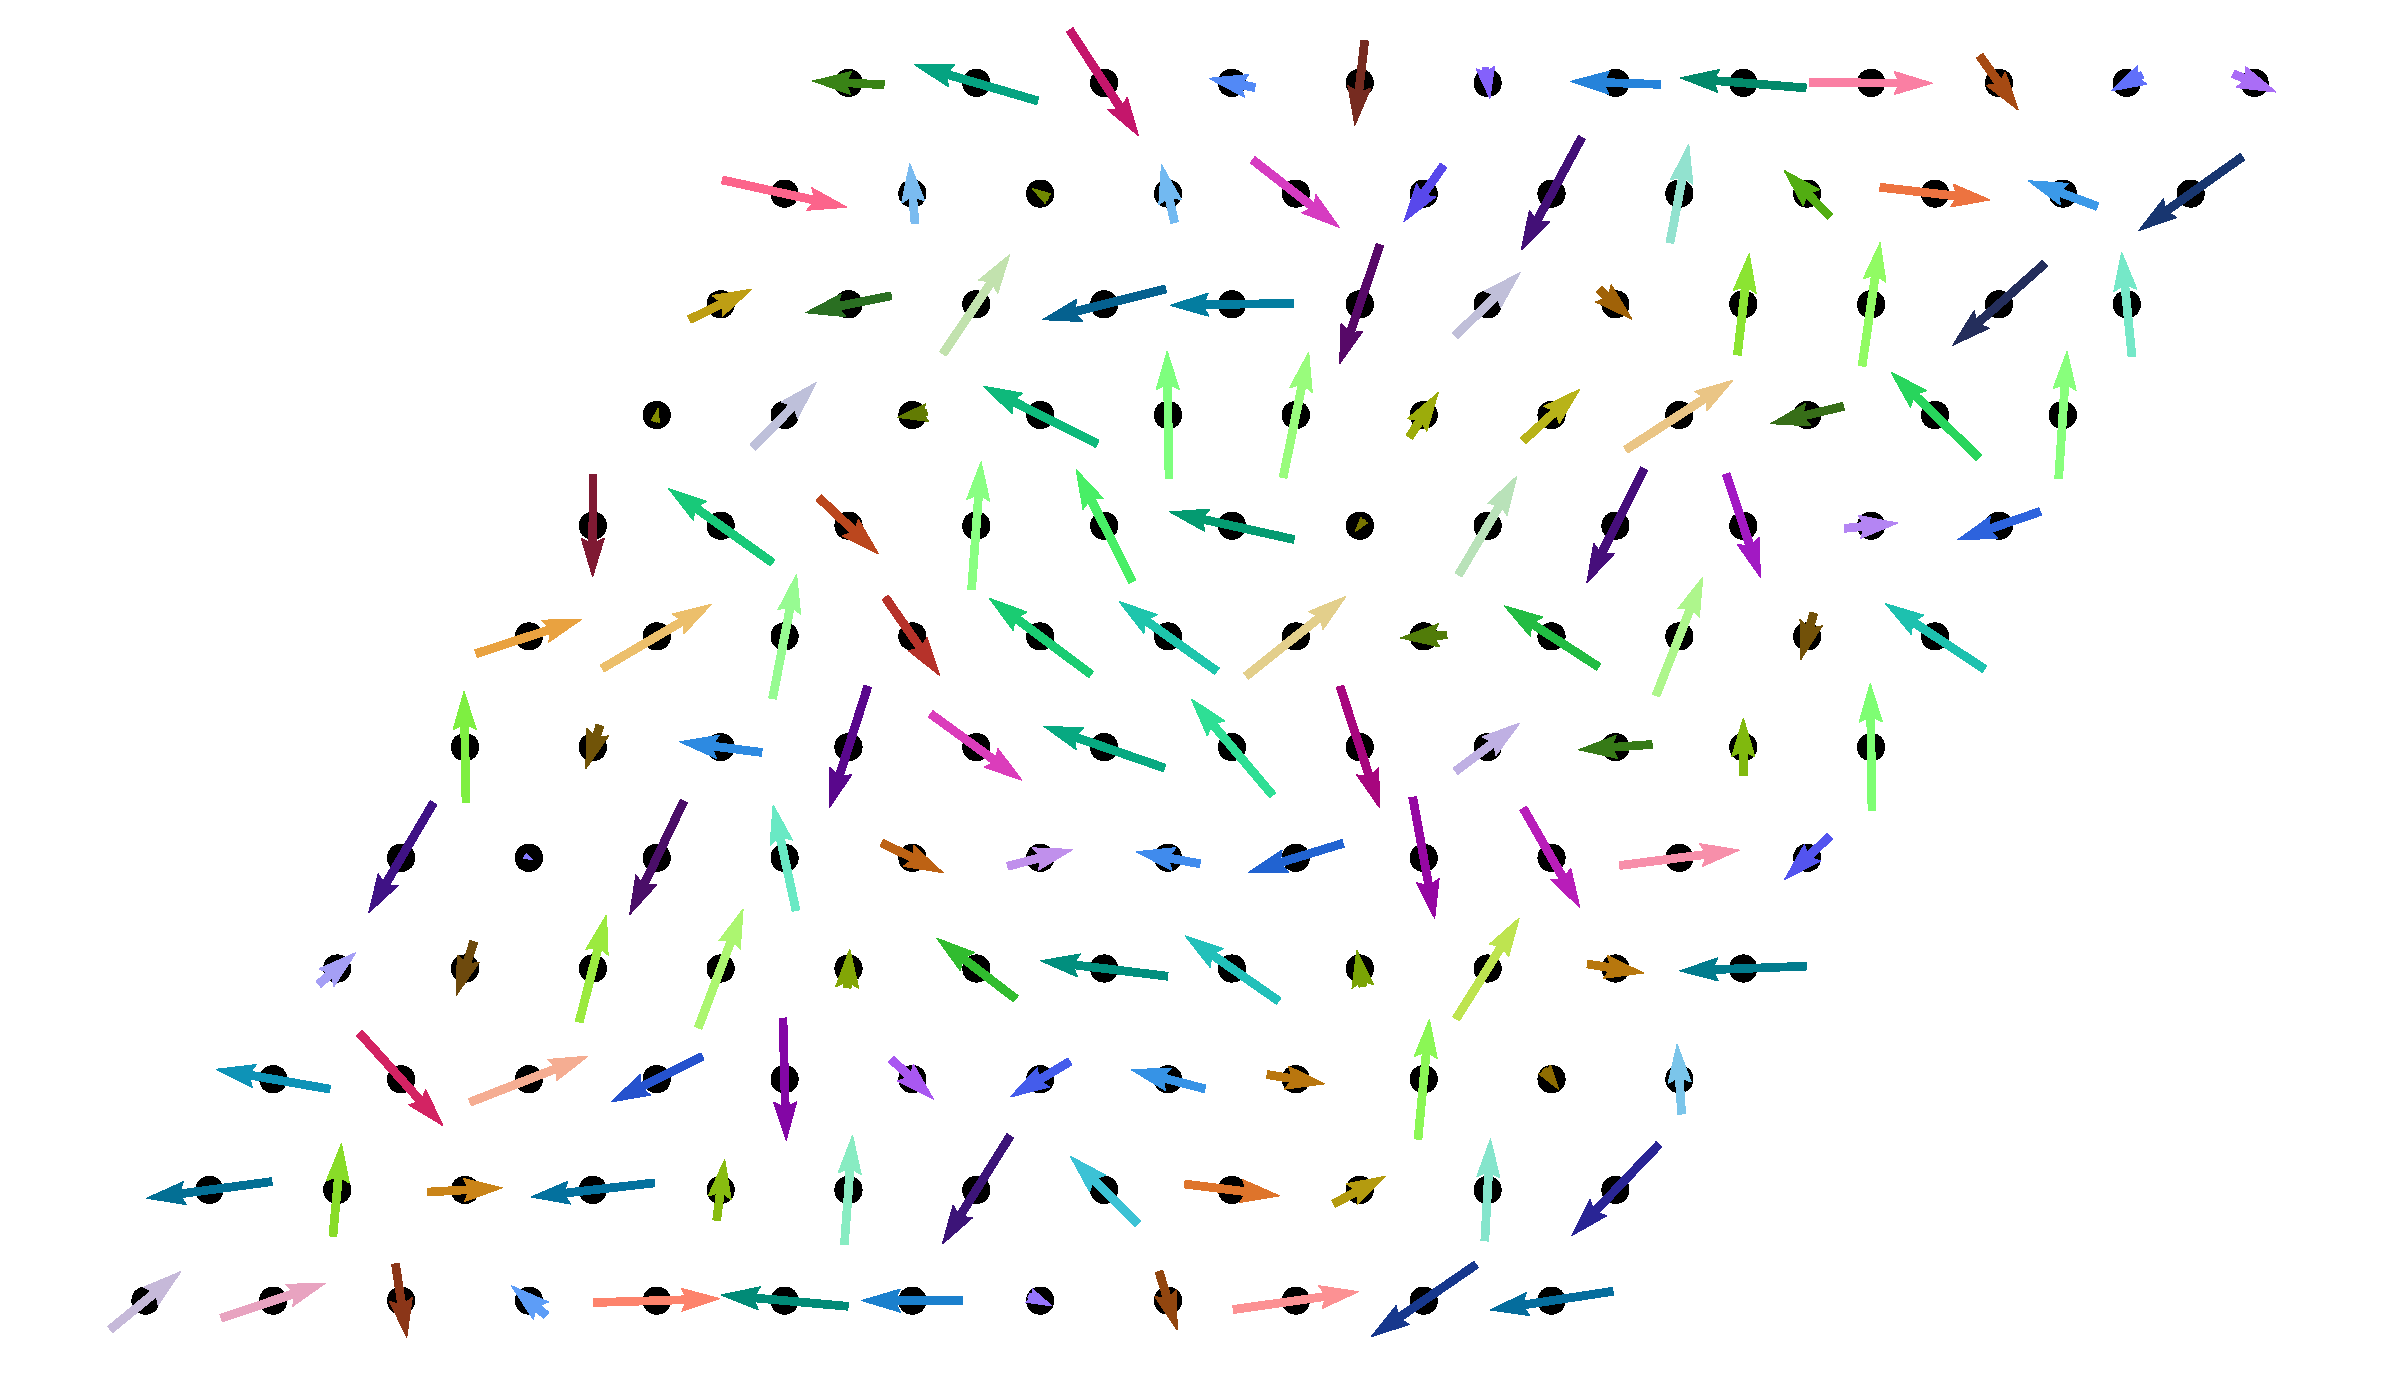
\includegraphics[width=0.45\textwidth]{FigA1.pdf}
    \caption{\label{fig:GSForPositiveGamma}(Color online) Typical disordered ground state for $J=K=0, \Gamma=1$. The 3D unit spin vectors were projected to the $xy$ plane and different vectors were represented by different colors.}
\end{figure}

\subsection{$J=K=0, \Gamma=-1$}
For pure ferromagnetic $\Gamma$ model, we found several energetically degenerate states as the classcial ground state, including FM state, stripe states and a noncollinear state. The ordered moment of the FM state along the $[111]$ direction. As for the stripe states, there are three degenerate spin configurations as shown in Fig.~\ref{fig:GSForNegativeGamma}(a)-(c) and the directions for the cyan, red, pink, green, yellow and blue arrows are $[\bar{1}11]$, $[1\bar{1}\bar{1}]$, $[1\bar{1}1]$, $[\bar{1}1\bar{1}]$, $[11\bar{1}]$ and $[\bar{1}\bar{1}1]$, respectively. Apart from these collinear states, a noncollinear state exist as the classical ground state. The magnetic unit-cell contains four lattice sites. The directions for the yellow, gray, pink, cyan arrows in Fig.~\ref{fig:GSForNegativeGamma}(d) are $[11\bar{1}]$, $[111]$, $[1\bar{1}1]$ and $[\bar{1}11]$, respectively.
\begin{figure}
    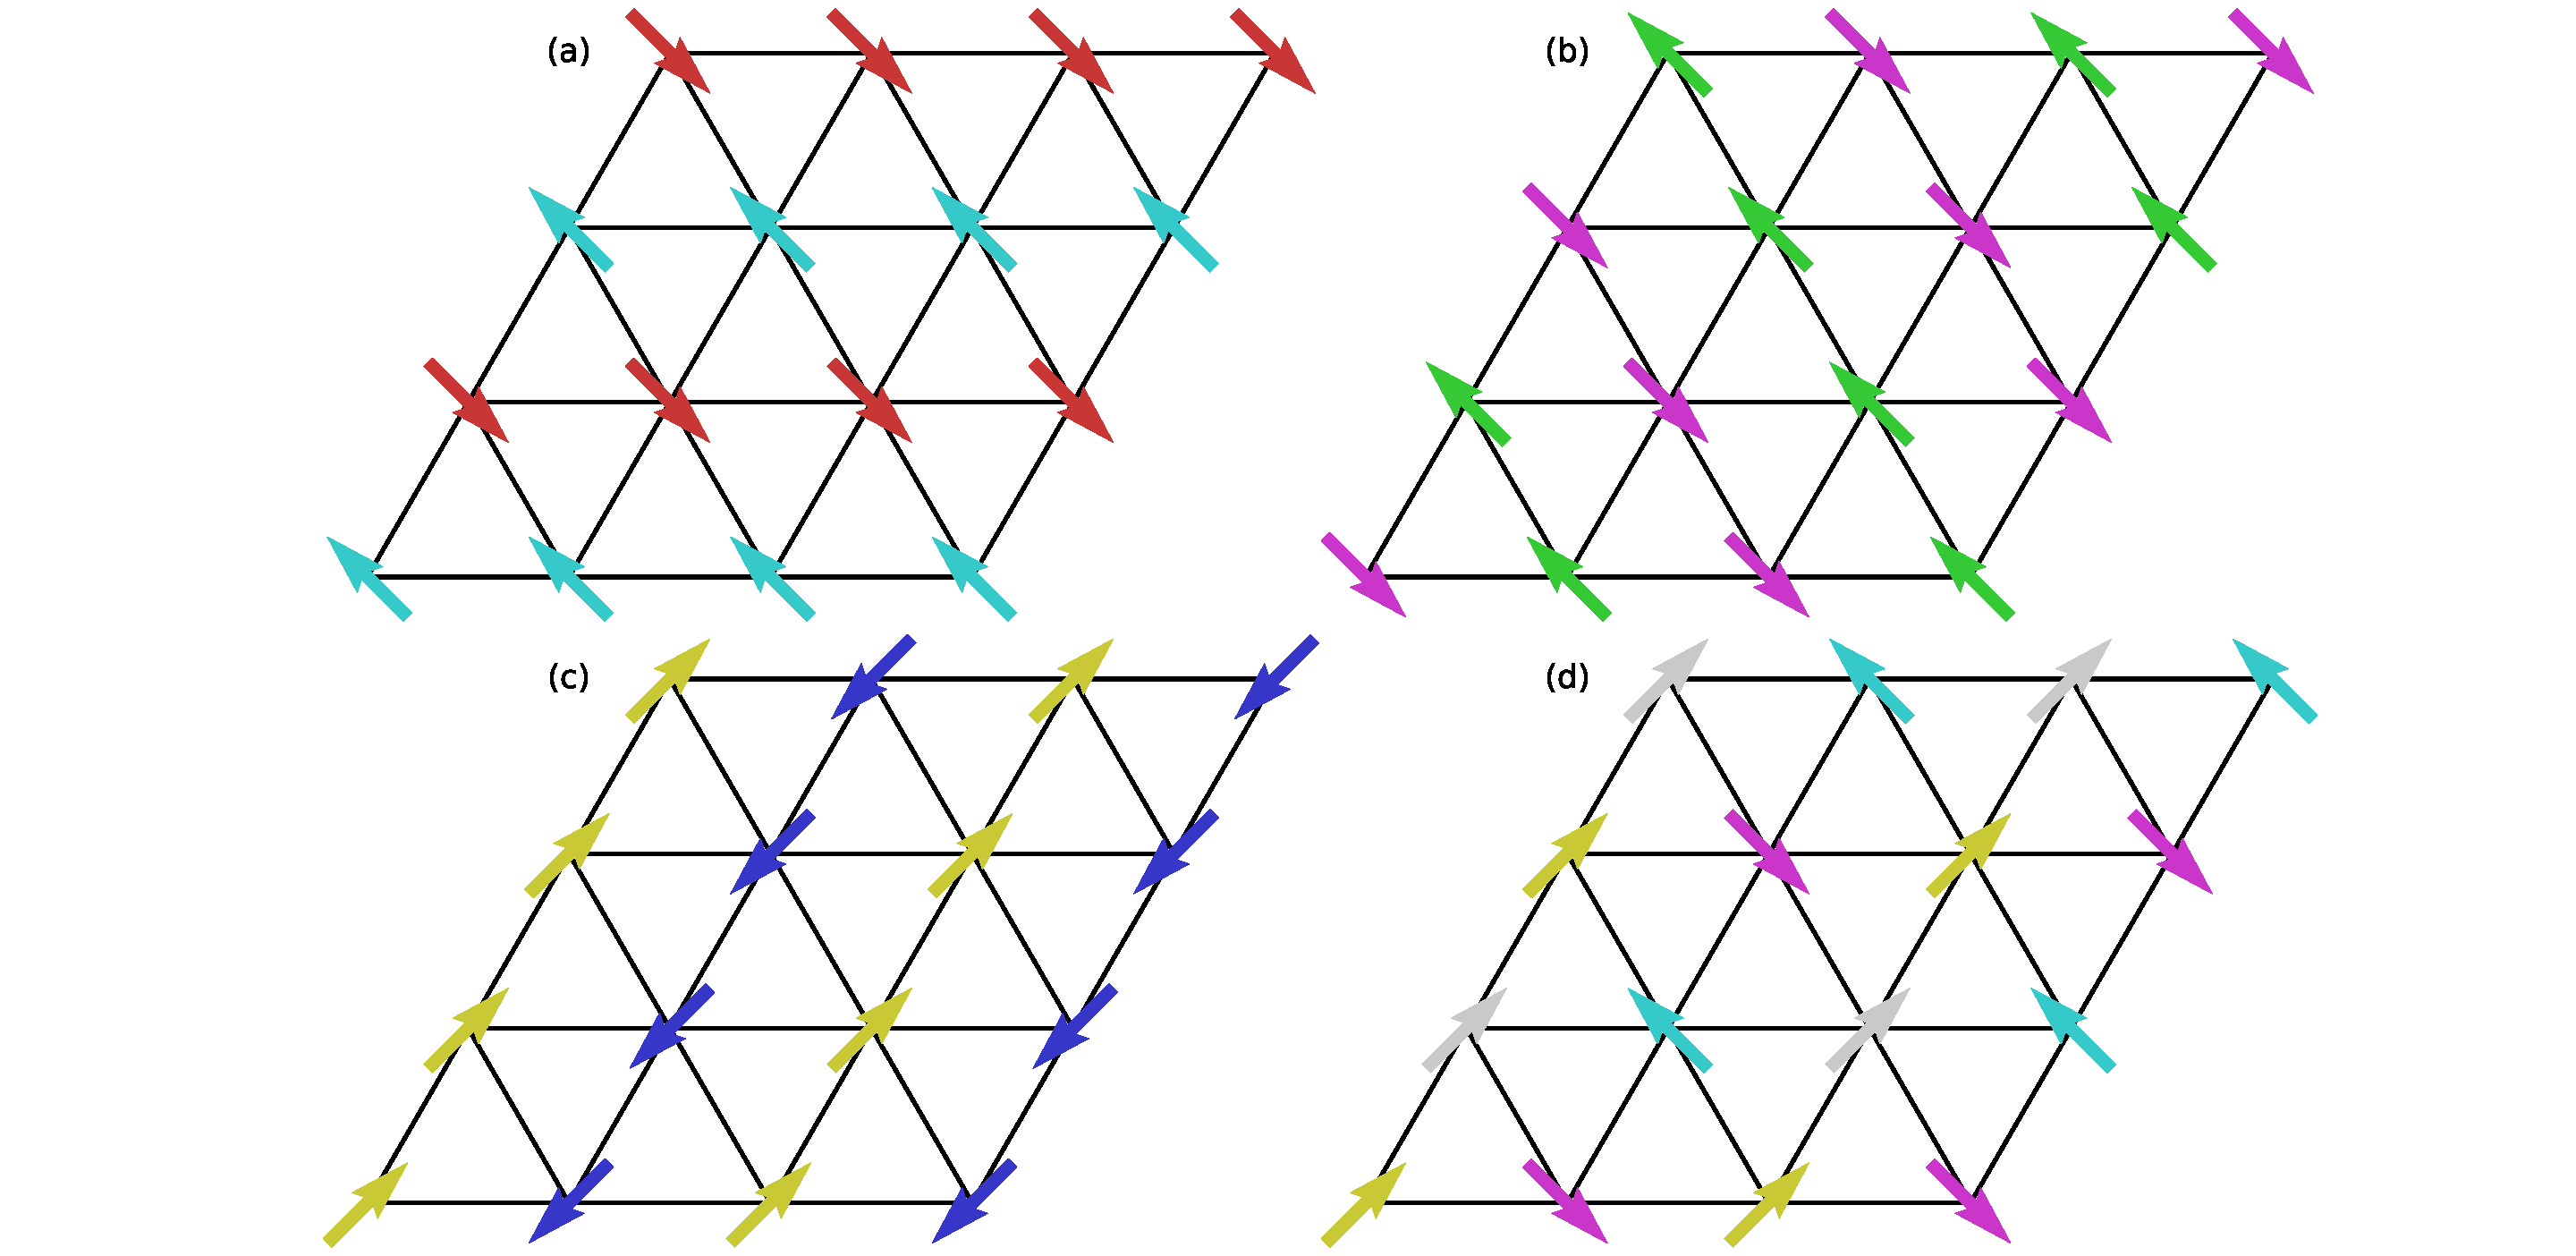
\includegraphics[width=0.45\textwidth]{FigA2.pdf}
    \caption{\label{fig:GSForNegativeGamma}(Color online) Typical ground state spin configurations for $J=K=0, \Gamma=-1$. The 3D unit spin vectors were projected to the $xy$ plane and different vectors were represented by different colors. (a)-(c) Stripe ordered states. The directions for the cyan, red, pink, green, yellow and blue arrows are $[\bar{1}11]$, $[1\bar{1}\bar{1}]$, $[1\bar{1}1]$, $[\bar{1}1\bar{1}]$, $[11\bar{1}]$ and $[\bar{1}\bar{1}1]$, respectively. (d) Noncollinear state. The directions for the yellow, gray, pink, cyan arrows are $[11\bar{1}]$, $[111]$, $[1\bar{1}1]$ and $[\bar{1}11]$, respectively.}
\end{figure}

\subsection{$J=\Gamma=0, K=1$}
The ground state for the classical antiferromagetic Kitaev model is also degenerate involving three nematic ordered states and three stripe ordered states. For the nematic ordered state shown in Fig.~\ref{fig:GSForPositiveK}(a), the spins on the chains along the $x$-bond direction form antiferromagetic chains and the direction for the orange arrow is $[100]$. There is no association between different chains. Similarly, the antiferromagetic chains along the $y$-bond and $z$-bond direction for Fig.~\ref{fig:GSForPositiveK}(b) and Fig.~\ref{fig:GSForPositiveK}(c) respectively. The direction for the orange arrow in Fig.~\ref{fig:GSForPositiveK}(b) is $[010]$ and in Fig.~\ref{fig:GSForPositiveK}(c) is $[001]$. In addition to these nematic ordered states, there are stripe ordered states that have the same energy as the nematic ordered states. For the stripe ordered states shown in Fig.~\ref{fig:GSForPositiveK}(d)-(f), the corresponding ordered moment lie in the $yz$, $xz$ and $xy$ plane, respectively.
\begin{figure}
    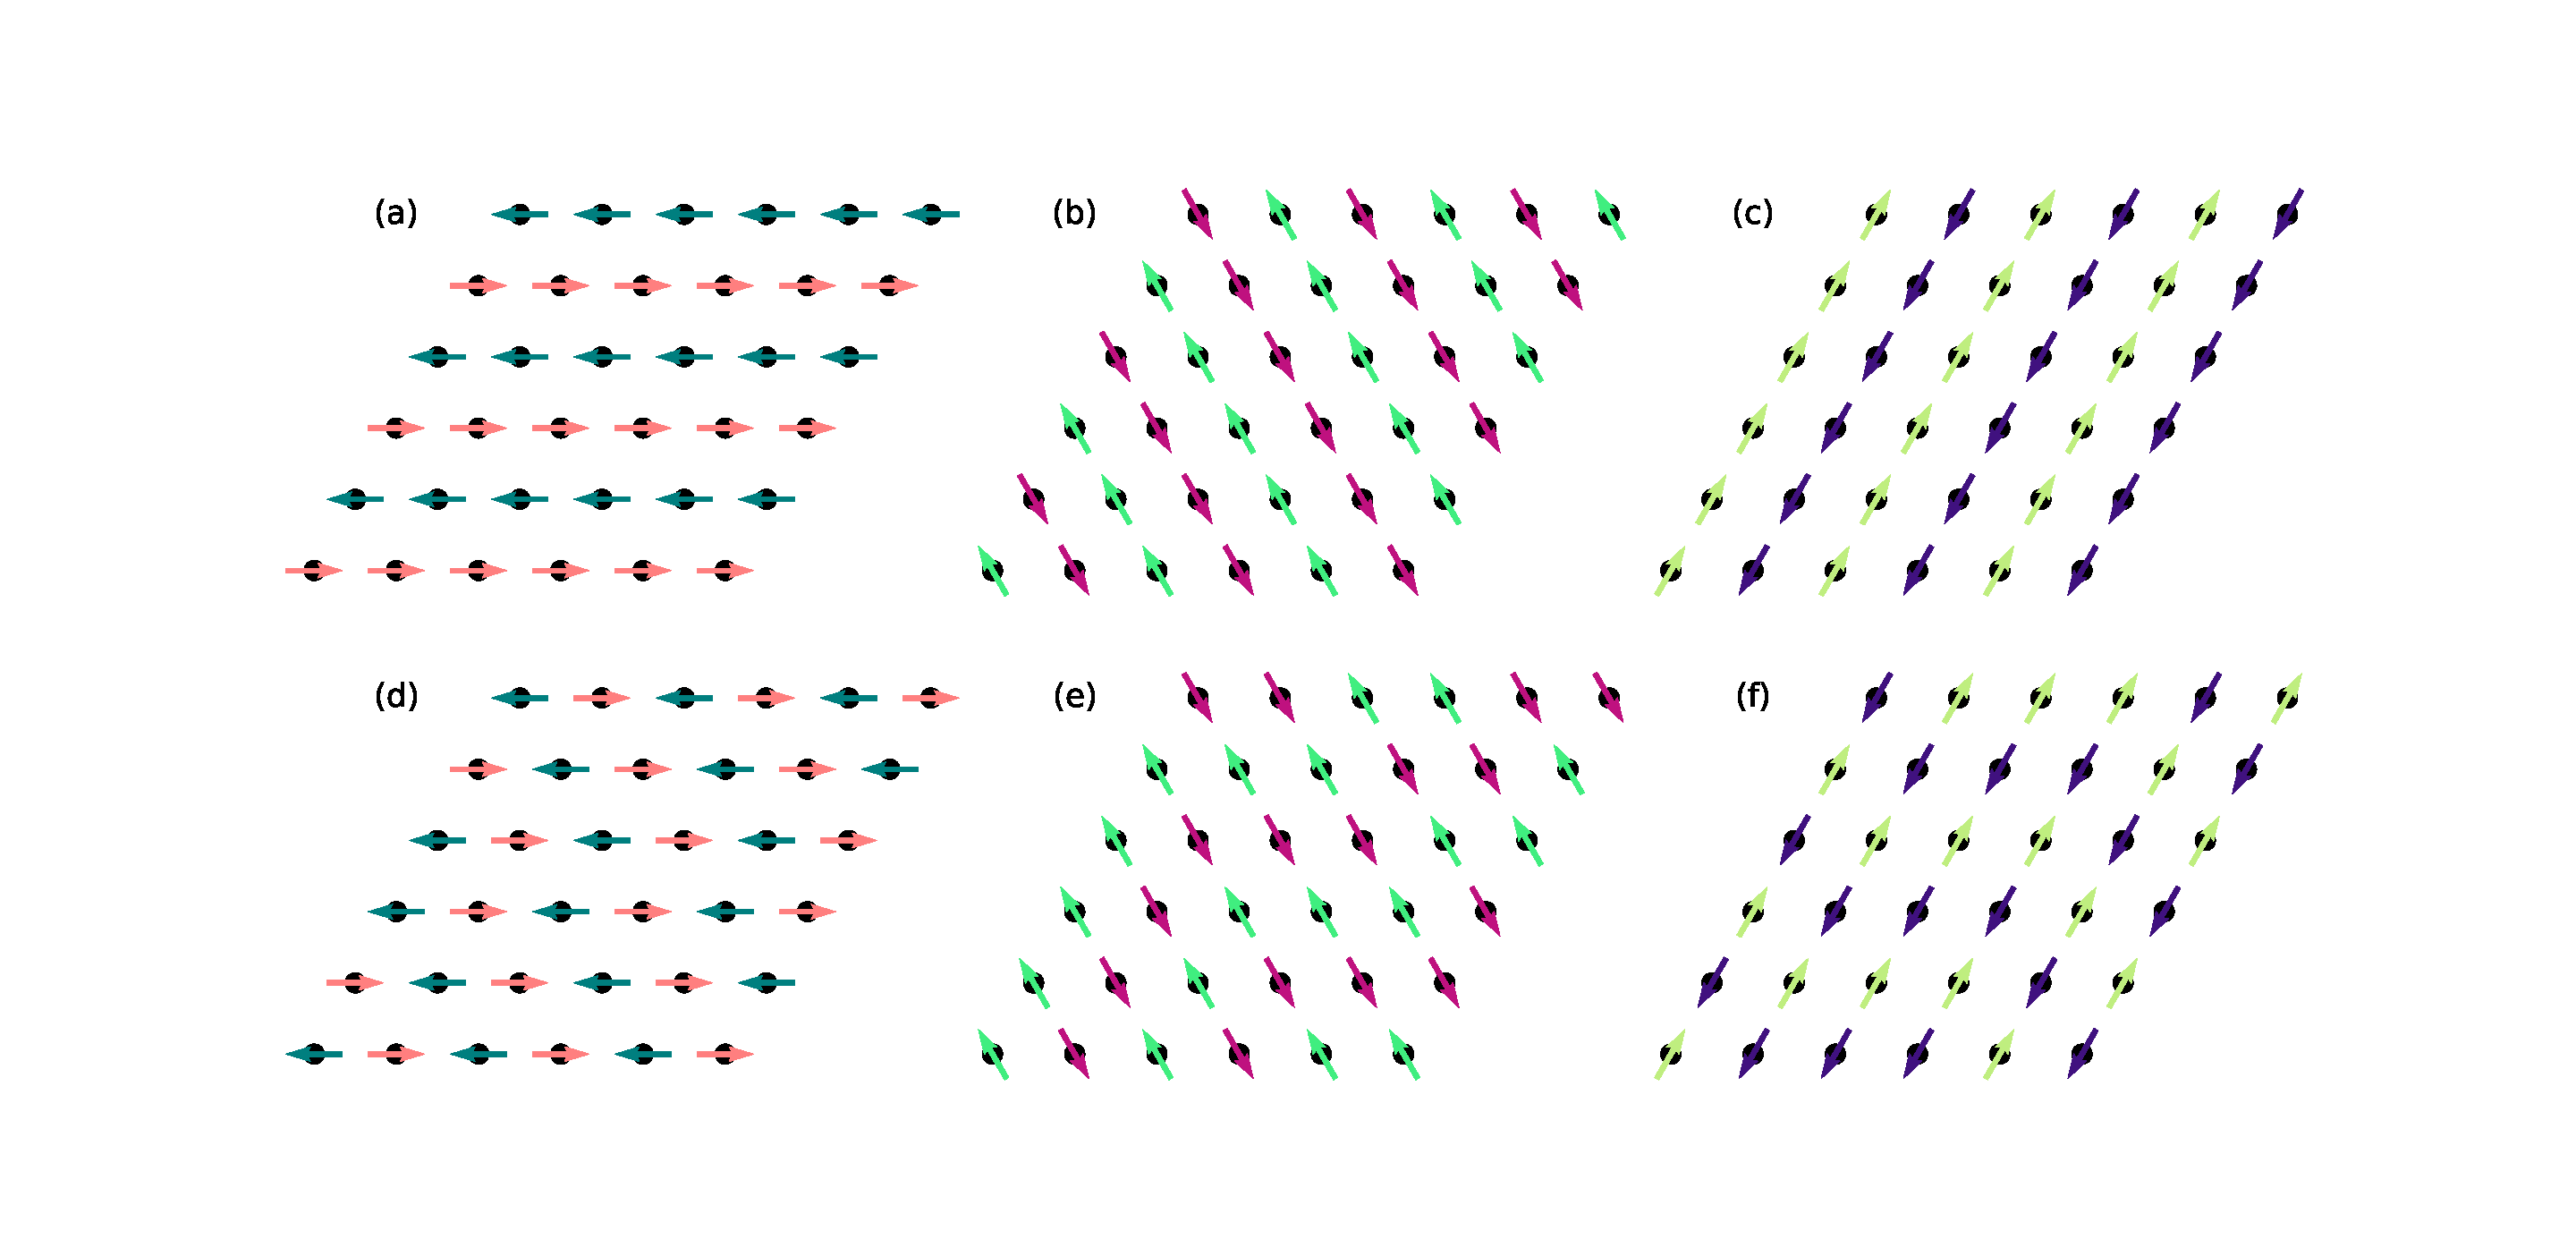
\includegraphics[width=0.5\textwidth]{FigA3.pdf}
    \caption{\label{fig:GSForPositiveK}(Color online) Nematic and stripe ground state spin configurations for $J=\Gamma=0, K=1$.}
\end{figure}

\section{\label{apx:AppendixB}Classical energy and moment direction of the stripe ordered states}
For classical stripe ordered states, all the spins are collinear and there are three degenerate spin configurations as shown in Fig.~\ref{fig:PhaseDiagram}(b)-(d) in the main text. The corresponding energies of the classical $J-K-\Gamma$ model for these spin configurations are
\begin{subequations}
    \begin{eqnarray}
        E_{StripeX}^{c} & = & -(J + K) + 2 K v^x v^x \nonumber \\
            & & +\: 2 \Gamma (v^y v^z - v^z v^x - v^x v^y)
            \label{eq:AEcStripeX} \\
        E_{StripeY}^{c} & = & -(J + K) + 2 K v^y v^y \nonumber \\
            & & +\: 2 \Gamma (v^z v^x - v^x v^y - v^y v^z)
            \label{eq:AEcStripeY} \\
        E_{StripeZ}^{c} & = & -(J + K) + 2 K v^z v^z \nonumber \\
            & & +\: 2 \Gamma (v^x v^y - v^y v^z - v^z v^x)
            \label{eq:AEcStripeZ}
    \end{eqnarray}
\end{subequations}
where $v^x$, $v^y$, $v^z$ are the corresponding components of the classical spin vector. The ordered moment direction of the classical stripe order is determined by the anisotropic parameters $K$ and $\Gamma$ and can be obtained by finding the global minimum of $E_{StripeX}^{c}$, $E_{StripeY}^{c}$ and $E_{StripeZ}^{c}$ with the constraint $|\bm{v}|=1$. It is clear from Eq.~\eqref{eq:AEcStripeX}, Eq.~\eqref{eq:AEcStripeY} and Eq.~\eqref{eq:AEcStripeZ}, if $\bm{v}_{min}$ minimize the energy, then $-\bm{v}_{min}$ also minimize the energy. Here we only consider one of the direction.

When $\Gamma=0$, it can be clearly seen from Eq.~\eqref{eq:AEcStripeX}, $E_{StripeX}^c$ takes minimum value at $v^x=0$ for positive $K$ and $v^x=1$ for negative $K$. When the $\Gamma$ interaction is included, the problem becomes a little more complex. To find the unit vector $\bm{v}_{min}$ that minimize $E_{StripeX}^{c}$, we use the Lagrange multiplier method. For $\Gamma>0, K=0$, $E_{StripeX}^{c}$ takes minimum value when the condition $v^x=v^y+v^z$ is fulfilled. On the other hand, when $\Gamma<0, K=0$, there are only two vectors that minimize $E_{StripeX}^{c}$, i.e., $v^y=v^z=-v^x=\pm 1/\sqrt{3}$.

More generally, if both $K, \Gamma \neq 0$, $E_{StripeX}^{c}$ has six extreme points where the first derivatives with respect to $v_x$, $v_y$ and $v_z$ equal zero. Here we give three of them explicitly and the other three are opposite to the given ones
\begin{subequations}
    \begin{eqnarray}
        & \bm{v}_0: \quad v_{0}^{y}=-v_{0}^{z} = 1/\sqrt{2}, & v_{0}^{x} = 0 \\
        & \bm{v}_1: \quad v_{1}^{y}=v_{1}^{z} = f_{1}(K, \Gamma), & v_{1}^{x} = g_{1}(K, \Gamma) v_{1}^{y} \\
        & \bm{v}_2: \quad v_{2}^{y}=v_{2}^{z} = f_{2}(K, \Gamma), & v_{2}^{x} = g_{2}(K, \Gamma) v_{2}^{y}
    \end{eqnarray}
\end{subequations}
and
\begin{subequations}
    \begin{eqnarray}
        \lambda_{1} & = &- (\Gamma +2 K - \sqrt{9\Gamma^2 - 4 \Gamma K + 4 K^2}) / 4 \nonumber \\
        \lambda_{2} & = & -(\Gamma +2 K + \sqrt{9\Gamma^2 + 4 \Gamma K + 4 K^2}) / 4 \nonumber \\
        f_{1,2}(K, \Gamma) & = & \frac{|\Gamma|}{\sqrt{4 \lambda_{1,2} (\lambda_{1,2} + \Gamma) + 3 \Gamma^{2}}} \\
        g_{1,2}(K, \Gamma) & = & (2 \lambda_{1,2} + \Gamma) / \Gamma
    \end{eqnarray}
\end{subequations}
For a specific $K$ and $\Gamma$, by comparing the values of $E_{StripeX}^{c}$ at $\bm{v}_0$, $\bm{v}_1$ and $\bm{v}_2$ we can determine the global minimum of $E_{StripeX}^{c}$ and the corresponding $\bm{v}_{min}$. When both $\Gamma$ and $K$ are positive, $E_{StripeX}^{c}$ takes minimum value at the direction determined by $\bm{v}_0$. Otherwise, $\bm{v}_1$ specifies the direction where $E_{StripeX}^{c}$ has lowest energy.

The similar analysis can be applied to $E_{StripeY}^{c}$ and $E_{StripeZ}^{c}$ and the ordered moment direction that minimize the classical energy can be obtained by a cyclic permutation $x \rightarrow y \rightarrow z \rightarrow x$ of the results for $E_{StripeX}^{c}$.



\newpage

\bibliography{ref}

\end{document}
